%  LaTeX support: latex@mdpi.com
%  For support, please attach all files needed for compiling as well as the log file, and specify your operating system, LaTeX version, and LaTeX editor.

%=================================================================
\documentclass[journal,article,submit,pdftex,moreauthors]{Definitions/mdpi}
\usepackage{url}
% Avoid fancyhdr warnings (MDPI template can require a taller header box).
\setlength{\headheight}{19pt}

% Below journals will use ACS reference format - This is the default for most MDPI journals
% We will use standard ACS format for this submission

%=================================================================
% MDPI internal commands - do not modify
\firstpage{1}
\makeatletter
\setcounter{page}{\@firstpage}
\makeatother
\pubvolume{1}
\issuenum{1}
\articlenumber{0}
\pubyear{2025}
\copyrightyear{2025}
\datereceived{ }
\daterevised{ } % Comment out if no revised date
\dateaccepted{ }
\datepublished{ }
% Some mdpi.cls versions do not define \hreflink; keep compilation robust.
\providecommand{\hreflink}[1]{}
% Compatibility shims (some mdpi.cls templates omit these metadata helpers).
\providecommand{\TitleCitation}[1]{}
\providecommand{\AuthorCitation}[1]{}
\providecommand{\orcidA}[1]{}
\hreflink{https://doi.org/} % If needed use \linebreak

%=================================================================
% Full title of the paper (Capitalized)
\Title{Privacy-Preserving Federated Learning for Secure Emergency Triage with a Multi-Modal Fusion Network with Multi-Head Self-Attention}

% MDPI internal command: Title for citation in the left column
\TitleCitation{Privacy-Preserving Federated Learning for Secure Emergency Triage with a Multi-Modal Fusion Network with Multi-Head Self-Attention}

% Author Orchid ID: enter ID or remove command
\newcommand{\orcidauthorA}{0000-0000-0000-000X} % Add \orcidA{} behind the author's name

% Authors, for the paper (add full first names)
\Author{Cenab Batu Bora $^{1}$\orcidA{}}

% MDPI internal command: Authors, for metadata in PDF
\AuthorNames{Cenab Batu Bora}

% MDPI internal command: Authors, for citation in the left column
\AuthorCitation{Bora, C.B.}

% Affiliations / Addresses
\address{%
$^{1}$ \quad Independent Researcher, Edmonton, AB T6G 2R3, Canada; cenab@ualberta.ca}

% Contact information of the corresponding author
\corres{Correspondence: cenab@ualberta.ca}

% Abstract
\abstract{Emergency department (ED) triage models benefit from multi-site data, but privacy regulations and security concerns often prevent pooling patient records across hospitals. We present a federated learning (FL) pipeline for emergency triage that trains a lightweight multi-modal attention model locally at each site and aggregates only model updates. The training objective is safety-aware: it combines class-balanced cross-entropy with a focal component and explicit penalties for under-triage of the critical band (ESI-1/ESI-2). The model footprint is under 0.3~MB (67.9k--70.1k parameters; FP32), enabling resource-constrained edge deployment. We evaluate on 558,029 encounters labeled with the 5-level Emergency Severity Index (ESI). A centralized ESI-5 neural model reaches 85.4\% test accuracy with 95.3\% critical-band sensitivity. In a cross-silo setting that uses the dataset's hospital-department identifier as three real sites, a flat FedAvg baseline (3 sites/clients, 20 rounds) achieves 75.3\% accuracy and 80.2\% critical sensitivity, while a red-focus hierarchical variant improves to 80.5\% accuracy and 90.8\% critical sensitivity. We add strong tabular baselines: HistGradientBoosting reaches 89.5\% accuracy and 91.5\% macro-F1. We also evaluate Byzantine resilience: under a simulated poisoning attack (29\% malicious clients, non-IID; 7 clients, 10 rounds), FedAvg accuracy drops to 61.4\% with 36.8\% over-triage, while coordinate-wise median aggregation recovers 80.8\% accuracy with 10.0\% over-triage. Finally, we report an optional differentially private mode (DP-SGD): in a 3-site, 5-round run with $\sigma=1.0$ and $\delta=10^{-5}$, RDP accounting yields $\varepsilon\approx1.15$ (max client, composed across rounds) and 84.3\% test accuracy, but the model fails on the rarest class (ESI-1 recall 0.0; macro-F1 68.3\%). These results clarify the safety--privacy--robustness trade-offs of federated triage and provide an open, reproducible baseline for future work on robust and private collaboration in emergency care.}

% Keywords
\keyword{federated learning; edge AI; privacy-preserving; healthcare analytics; differential privacy; trustworthy AI; secure aggregation; emergency triage; multi-modal learning; clinical safety}

%=================================================================
\begin{document}

%%%%%%%%%%%%%%%%%%%%%%%%%%%%%%%%%%%%%%%%%%
\section{Introduction}\label{sec:intro}

Emergency departments (EDs) face the constant challenge of quickly and accurately identifying patients who need immediate care amid overwhelming demand. In the United States alone, EDs handle over 155 million visits annually, with 11.5\% resulting in hospital admissions and 2\% requiring critical care unit transfers \cite{cdc2022}. Delays and mis-triage, particularly under-triage of critical cases, can delay time-sensitive interventions. While machine learning has shown promise for improving triage, building effective models requires large, diverse datasets. This presents a significant hurdle, as privacy regulations like HIPAA and GDPR often prevent hospitals from pooling their data \cite{voigt2017}. These data silos ultimately hinder the development of more robust, collaborative models. As a potential solution, Edge AI allows us to bring the computation to the data itself. By treating each hospital as a local edge node, we can use federated learning to collaboratively train a shared model without ever exchanging raw patient records. Instead, only model parameters are sent to a central server for aggregation \cite{mcmahan2017,kairouz2021}, which can satisfy regulatory requirements while still enabling real-time intelligence at the point of care.

It is important to recognize, however, that federated learning is not inherently private. The exchange of gradients can inadvertently leak sensitive information through techniques such as gradient inversion and membership inference \cite{zhu2019deep,shokri2017}. Federated systems are also susceptible to Byzantine attacks, where malicious clients poison the global model by contributing adversarial updates \cite{blanchard2017,yin2018byzantine}. These vulnerabilities motivate additional safeguards beyond the basic federated learning protocol.

To address these challenges, we design a federated learning framework for emergency triage that prioritizes clinical safety and supports optional privacy and integrity mechanisms. Our framework allows multiple hospitals to collaboratively train a shared triage model without exchanging raw patient records. Our contributions include a lightweight, multi-path attention architecture that is well-suited for edge deployment, a safety-aware hierarchical learning approach that minimizes dangerous under-triage of the critical band, and a federated pipeline with optional client-side differential privacy (DP-SGD) and robust aggregation. In addition, we implement post-hoc calibration and decision-focused thresholding to ensure that predicted probabilities are reliable and clinically usable. To further enhance trustworthiness, we provide evaluation outputs covering fairness diagnostics, interpretability hooks, and reliability metrics, and we release an open, reproducible toolkit to support further research.

We evaluate our approach using a dataset of 558,029 emergency department encounters, each labeled with the Emergency Severity Index (ESI), a validated 5-level triage scale. Missing values are imputed using training-set medians, and we reserve a held-out validation set for calibration and operating-point selection. For our analysis, we adopt an 80/10/10 stratified split (seed 42): 80\% training, 10\% validation, and 10\% held-out testing.

Our centralized baseline neural model achieves 85.4\% test accuracy with 95.3\% critical-band sensitivity. In cross-silo federated learning using the dataset's three hospital-department partitions as real sites, a flat FedAvg baseline (3 sites/clients, 20 rounds) reaches 75.3\% accuracy and 80.2\% critical sensitivity, while a red-focus hierarchical variant improves to 80.5\% accuracy and 90.8\% critical sensitivity (13.3\% under-triage vs.\ 21.7\% for the flat baseline). When DP-SGD is enabled (3 sites, 5 rounds; $\sigma=1.0$; $\delta=10^{-5}$), RDP accounting yields a composed privacy budget of $\varepsilon\approx1.15$ (max client) and 84.3\% test accuracy, but the DP model fails on the rarest class (ESI-1 recall 0.0), which reduces macro-F1 (68.3\%) and critical sensitivity (78.1\%). Communication overhead is small: with a 0.27--0.28~MB FP32 model, each client exchanges roughly 0.54--0.56~MB per round (uplink+downlink), and the total system communication is roughly 1.63--1.68~MB per round for three clients.

Our results show that safety-aware federation can recover much of the centralized utility without pooling data, but formal differential privacy introduces a sharp privacy--utility trade-off in our multi-class triage setting. We implement and empirically evaluate robust aggregation (median/trimmed-mean) against simulated Byzantine clients: under a poisoning attack, FedAvg suffers a large accuracy drop and a sharp increase in over-triage, while median aggregation recovers much of the utility and reduces attack-induced over-triage. While fully centralized models and strong tabular baselines can achieve higher accuracy, our federated approach reduces direct data movement and has minimal communication requirements, confirming its suitability for deployment in resource-constrained edge environments.

The remainder of this paper is organized as follows. Section~\ref{sec:related} reviews related work in ED triage modeling, federated learning in healthcare, privacy-preserving techniques, and security considerations. Section~\ref{sec:methods} presents our methodology, including the dataset, model architecture, safety-aware training objective, federated learning protocol, and privacy mechanisms. Section~\ref{sec:experiments} describes the experimental setup and evaluation metrics. Section~\ref{sec:results} reports our results, emphasizing privacy-utility trade-offs, calibration quality, safety metrics, and trustworthiness evaluation. Section~\ref{sec:discussion} discusses security and privacy implications, limitations, and future directions. Finally, Section~\ref{sec:conclusion} concludes the paper.

%%%%%%%%%%%%%%%%%%%%%%%%%%%%%%%%%%%%%%%%%%
\section{Related Work}\label{sec:related}

\subsection{Emergency Department Triage Modeling}

Early machine learning approaches to emergency department triage have shown that routinely available signals, such as vitals, demographics, and chief complaints, can outperform conventional rule-based systems like the Emergency Severity Index in predicting critical outcomes and hospitalization \cite{raita2019,levin2018,liu2021_sci_rep}. Large-scale studies using decision-curve analysis have also reported net-benefit gains, which indicates clinical utility for risk stratification. Subsequent systems have integrated structured features with chief-complaint text or clinical notes, improving both discrimination and calibration \cite{chang2024_bmc}. Attention-based architectures have also been explored for triage modelling \cite{gligorijevic2018}.

Recent systematic reviews from 2024 and 2025 have highlighted the growing role of machine learning and natural language processing in emergency department triage. At the same time, these reviews also emphasize the persistent challenges of under-triage and over-triage, as well as the need for decision-focused metrics that go beyond the traditional AUROC. Our work builds on this foundation but differs in three key aspects. First, we encode feature groups as tokens and fuse them using a lightweight attention mechanism, which allows us to capture interactions between different groups of features. Second, we optimize a clinically cost-sensitive objective that is specifically designed to reduce critical under-triage. Finally, we transpose our entire pipeline to a federated setting, which allows us to preserve calibration and incorporate privacy safeguards.

\subsection{Safety-Aware Learning and Decision-Focused Evaluation}

It's clear that metrics like accuracy and AUROC don't tell the whole story. For clinical adoption, we need to consider explicit cost trade-offs and make careful choices about the operating point. Decision curve analysis (DCA), for example, offers a principled way to compare the net benefit of different models across a range of decision thresholds \cite{vickers2006}. In a similar vein, cost-sensitive learning formalizes the asymmetric penalties of mis-triage by using class-weighted or instance-weighted objectives \cite{araf2024_csl_review,pes2021_cost_sens_med}. As another tool, Neyman-Pearson (NP) classification can prioritize one type of error while constraining another \cite{tong2013_np}.

Our hierarchical critical-first architecture is a pragmatic way of putting this safety-first principle into practice. It is paired with a clinical penalty matrix and post-hoc threshold selection under recall constraints, a combination that ensures the model prioritizes critical cases without sacrificing an acceptable level of overall performance.

\subsection{Calibration and Reliability Under Distribution Shift}

In the context of clinical decision-making, calibrated probabilities are essential for threshold selection and expected-cost minimization. Temperature scaling is a strong post-hoc calibration method \cite{guo2017}, but calibration can degrade under dataset shift \cite{ovadia2019,yu2022_mdt}. To address this, we report negative log-likelihood (NLL), expected calibration error (ECE), and Brier score in addition to accuracy and F1-score, and we select operating points on a held-out validation set.

\subsection{Federated Learning in Healthcare}

Federated learning offers a way to train models across multiple sites without sharing raw patient data \cite{mcmahan2017,kairouz2021}. In healthcare, federated learning has been explored for outcome prediction across institutions and modalities \cite{rieke2020,sheller2020,dayan2021}. Systematic reviews through 2024 identify hundreds of applications but note that relatively few have reached real-world deployment \cite{teo2024_fl_survey}; reporting on calibration and decision thresholds also remains uncommon.

More recently, research has started to address calibration in federated learning more directly; for example, FedCal improves local and global calibration under heterogeneity \cite{peng2024_fedcal}. To address this gap in the context of triage applications, our pipeline incorporates post-aggregation temperature scaling and validation-time threshold selection with safety constraints.

\subsection{Privacy-Preserving Techniques in Federated Learning}

While federated learning reduces direct data exposure by keeping training data local, it is important to remember that model updates can still leak sensitive information \cite{zhu2019deep,shokri2017}. Differential privacy (DP) provides a formal framework for bounding privacy leakage \cite{dwork2006}. In practice, DP-SGD adds noise to clipped gradients during training \cite{abadi2016deep}, and modern accounting tools often use R\'enyi DP or related analyses \cite{mironov2017}.

DP-SGD can be deployed in both centralized and federated settings; practical implementations in PyTorch are available through Opacus \cite{yousefpour2021opacus}. Recent work also explores alternative DP definitions and accounting approaches (e.g., Gaussian DP) that can yield tighter privacy--utility trade-offs in some regimes \cite{bu2020}.

\subsection{Secure Aggregation and Byzantine Robustness}

Even with the protections of differential privacy, federated systems are still vulnerable to Byzantine attacks, where malicious clients contribute poisoned updates to degrade or bias the global model \cite{blanchard2017,yin2018byzantine}. Secure aggregation can reduce server visibility into individual client updates, for example via cryptographic protocols or related techniques \cite{bonawitz2017,zhang2020}.

Byzantine-robust aggregation, on the other hand, provides a defense against malicious clients through the use of statistical methods. Common approaches include coordinate-wise median and trimmed-mean \cite{yin2018byzantine}. Our pipeline implements median and trimmed-mean as alternatives to FedAvg \cite{mcmahan2017}. Although we do not evaluate targeted poisoning attacks in this work, these mechanisms provide a starting point for secure deployment.

\subsection{Trustworthy and Explainable AI in Distributed Settings}

Explainability and fairness are crucial for building trustworthy AI, especially in healthcare, where decisions can have a direct impact on patient outcomes. Post-hoc explanation methods such as SHAP and LIME can provide feature-level interpretations of model predictions \cite{lundberg2017,ribeiro2016}. Fairness metrics can be used to assess disparate impact across demographic groups, with frameworks such as equality of opportunity being commonly applied \cite{hardt2016}.

In federated settings, ensuring fairness across distributed populations can introduce additional challenges due to heterogeneity. Recent work on agnostic and distributionally robust federated learning addresses worst-case performance gaps across clients \cite{mohri2019agnostic}. We support subgroup fairness evaluation (accuracy/F1 and rate-based checks across age and gender) alongside optional SHAP analysis.

\subsection{Positioning Relative to Prior Work}

Our work unifies several research directions. Dayan et al. demonstrated healthcare FL for clinical outcomes, but did not study hierarchical safety heads, decision-focused threshold selection, or integrated DP mechanisms in the triage setting \cite{dayan2021}. Raita et al. established triage ML gains at scale using DCA, but their model was trained centrally and did not include federated training or a safety-first hierarchy \cite{raita2019}. Clinical deployments have shown improvements compared to traditional ESI, but often rely on centralized data, limiting scalability across institutions \cite{levin2018}. Finally, while the DP and FL literature provides foundational privacy and systems guidance \cite{dwork2006,kairouz2021}, there remains a gap in end-to-end, safety-focused triage systems with clinically interpretable calibration and operating-point selection.

In contrast, we provide a complete pipeline that integrates multi-modal attention, safety-aware hierarchical modeling, and privacy-preserving federated learning with differential privacy. Our pipeline also includes robust aggregation and calibrated operating points, and it is designed with end-to-end reproducibility and a comprehensive trustworthiness evaluation.

%%%%%%%%%%%%%%%%%%%%%%%%%%%%%%%%%%%%%%%%%%
\section{Methods}\label{sec:methods}

\subsection{Dataset and Feature Engineering}\label{sec:dataset}

Our analysis is based on a publicly available hospital triage dataset that contains 558,029 emergency department encounters. Each of these encounters is labeled with the Emergency Severity Index (ESI), a validated 5-level triage scale that ranges from ESI-5 (the lowest urgency) to ESI-1 (the highest urgency, indicating an immediate life-threatening condition). For the purpose of model training, we encode the ESI levels as integers, where $y \in \{0, 1, 2, 3, 4\}$ and $y = 5 - \text{ESI}$. In this encoding scheme, $y=0$ corresponds to ESI-5, and $y=4$ corresponds to ESI-1.

Because ESI-1 and ESI-5 are comparatively rare, we also report results on a 3-class operational mapping derived from ESI: Green = \{ESI-5, ESI-4\}, Yellow = \{ESI-3\}, and Red = \{ESI-2, ESI-1\}. This binning represents a coarse low/medium/high acuity triage decision and reduces label sparsity for the most extreme acuity levels.

Figure~\ref{fig:class-distribution} summarizes the label distribution for the full 5-class task and highlights the severe class imbalance at ESI-1 (0.9\% of encounters).

\begin{figure}[H]
\centering
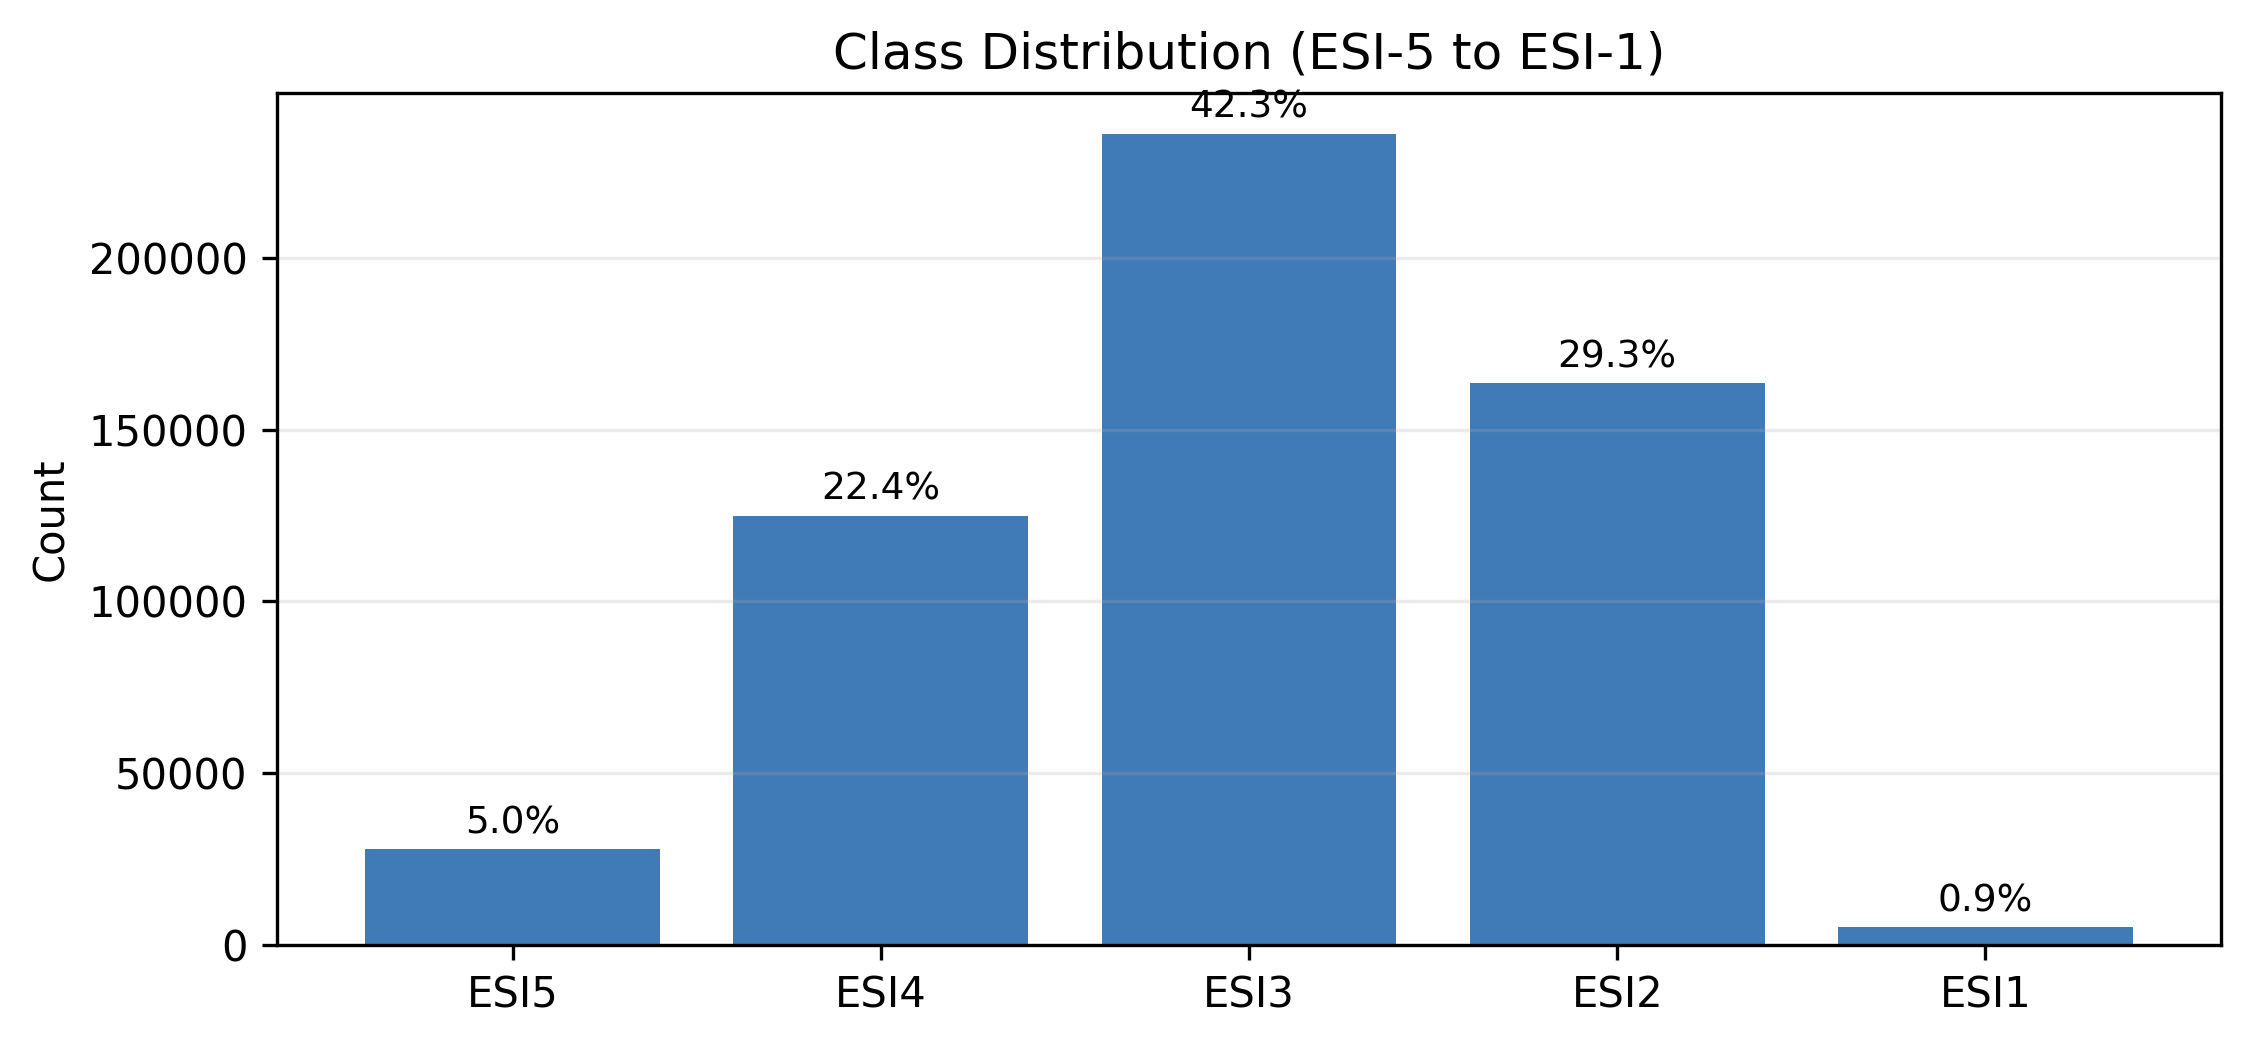
\includegraphics[width=0.9\textwidth]{figures/dataset_class_distribution.png}
\caption{Class distribution for ESI-5 (encoded as ESI-5 to ESI-1). ESI-1 is rare (0.9\%), which makes extreme-class recall and macro-averaged metrics particularly sensitive to modeling and operating-point choices.}
\label{fig:class-distribution}
\end{figure}

Through feature engineering, we have created six groups of inputs: vitals, symptoms, risk factors, context, labs, and interactions. The vitals group includes heart rate, systolic and diastolic blood pressure, respiratory rate, oxygen saturation (SpO$_2$), temperature, and age. The symptoms group consists of binary indicators that are derived from chief complaint flags, such as chest pain, shortness of breath, or altered mental status. The risk factors group includes the comorbidity count, prior emergency department visits, and chronic condition indicators. The contextual features group includes gender, arrival time features (such as the day of the week, the hour, and whether it was a holiday), and the mode of arrival. The lab features group is composed of recent laboratory values, such as glucose, creatinine, hemoglobin, and white blood cell count. Finally, the interaction features group contains engineered cross-features, such as age $\times$ heart rate or respiratory rate, which are designed to capture non-linear risk patterns.

To ensure consistency, missing values are imputed with per-feature medians computed on the training split. Where enabled, continuous features are also standardized using z-score normalization fitted on the training split. These statistics can be saved with the model checkpoints to ensure that the same preprocessing can be applied at inference time.

We use a stratified 80/10/10 split with a fixed random seed of 42. This means that 80\% of the data is used for training, 10\% for validation (including calibration and threshold selection), and the final 10\% for held-out test evaluation. In our federated experiments, the training split is partitioned across clients, while the validation and test sets remain global to ensure a consistent evaluation.

\subsection{Threat Model and Privacy Assumptions}\label{sec:threat_model}

We adopt an honest-but-curious server as our threat model. In this scenario, the central aggregator is assumed to follow the federated learning protocol correctly but may attempt to infer private information from the model updates it receives. While we assume that the clients are generally non-adversarial, we incorporate robust aggregation to provide resilience against potential outliers or malicious updates. Our security goals are fourfold. First, to ensure confidentiality, no raw patient data (Protected Health Information, or PHI) leaves the client sites; only model weight updates are communicated. Second, to protect privacy, model updates should not leak sensitive information about individual patients, and we employ differential privacy to provide formal guarantees for this. Third, to maintain integrity, the global model should be robust to anomalous or adversarial client updates, which we address by using robust aggregation to provide statistical defenses. Finally, to achieve secure communication, all client-server communications are protected with standard TLS encryption to prevent eavesdropping. In addition, secure aggregation protocols can be employed to ensure that the server only has access to the aggregated parameters.

For deployment, we recommend a combination of secure aggregation and always-on differential privacy, in addition to audit logging and model-card documentation. Our release of the software supports client-side DP-SGD and robust aggregation, and the integration of secure aggregation is a straightforward process that is compatible with our architecture.

\subsection{Model Architecture}\label{sec:architecture}

\subsubsection{Multi-Path Attention Network}

Each of the six feature groups is encoded by a dedicated multi-layer perceptron (MLP), producing a group embedding. If we let $g \in \{\text{vital}, \text{symptom}, \text{risk}, \text{context}, \text{lab}, \text{interaction}\}$ denote the six feature groups, then for each group $g$, the encoder maps the input $\mathbf{x}^{(g)} \in \mathbb{R}^{d_g}$ to an embedding, $\mathbf{h}^{(g)} = f_g(\mathbf{x}^{(g)}) \in \mathbb{R}^{d}$, where $f_g$ is a small MLP with ReLU activation and dropout.

We then stack the embeddings $\mathbf{H} = [\mathbf{h}^{(\text{vital})}; \mathbf{h}^{(\text{symptom})}; \dots; \mathbf{h}^{(\text{interaction})}] \in \mathbb{R}^{6 \times d}$ and apply multi-head self-attention to fuse information across feature groups:
\begin{equation}
\tilde{\mathbf{H}} = \text{MultiHeadAttention}(\mathbf{H}, \mathbf{H}, \mathbf{H}).
\end{equation}
The attended embeddings are pooled (mean pooling) to obtain a global representation $\bar{\mathbf{h}} \in \mathbb{R}^{d}$, and a compact MLP maps $\bar{\mathbf{h}}$ to logits $\mathbf{z} \in \mathbb{R}^{K}$, where $K=5$ for ESI-5 and $K=3$ for the binned Green/Yellow/Red setting.

At inference time, logits can be temperature-scaled, $\mathbf{z}' = \mathbf{z}/T$, and optionally adjusted with per-class offsets for operating-point tuning. Predicted probabilities are given by $\hat{\mathbf{p}} = \text{softmax}(\mathbf{z}')$.

The model footprint is small (67.9k--70.1k parameters; 0.27--0.28~MB in FP32 precision, i.e., 0.26--0.27~MiB), which supports low-latency inference on edge hardware and keeps federated communication modest. Each client transmits and receives approximately one model copy per round (uplink+downlink), corresponding to roughly 0.54--0.56~MB per client per round depending on the configuration.

\subsubsection{Hierarchical Ensemble for Safety-First Triage}

To prioritize the detection of critical cases, we generalize a hierarchical critical-first design to the ESI-5 scale. In this design, a gate head performs a binary classification to distinguish between non-critical cases (ESI-5, ESI-4, and ESI-3) and critical cases (ESI-2, and ESI-1). Two specialist heads then refine the predictions within each of these bands: a non-critical specialist performs a 3-way classification over the set \{ESI-5, ESI-4, ESI-3\}, and a critical specialist performs a 2-way classification over the set \{ESI-2, ESI-1\}.

The final probabilities are then composed as follows:
\begin{align}
P(y = c) &= P(\text{NonCrit}) \cdot P(c \mid \text{NonCrit}) \quad \text{if } c \in \{\text{ESI-5, ESI-4, ESI-3}\}, \\
P(y = c) &= P(\text{Crit}) \cdot P(c \mid \text{Crit}) \quad \text{if } c \in \{\text{ESI-2, ESI-1}\}.
\end{align}

This hierarchical structure allows the model to focus its specialized capacity on critical-band discrimination while still maintaining overall coverage. In this way, the gate head acts as a first-stage alarm system, which improves the model's sensitivity to high-acuity patients.

\subsection{Safety-Aware Training Objective}\label{sec:loss}

We train our model with a composite loss function that addresses class imbalance, hard example emphasis, clinical cost asymmetry, and explicit critical-miss penalties:

\begin{align}
\mathcal{L} &= \mathcal{L}_{\text{CE}} + w_{\text{focal}}\,\mathcal{L}_{\text{focal}}(\alpha=0.25, \gamma=2.0) \notag \\
&\quad + w_{\text{safety}}\,\mathbb{E}[M_{y,\hat{y}}] + w_{\text{crit}}\,\texttt{critical\_miss\_penalty}\cdot \mathbb{E}\!\left[\mathbf{1}[y \in \mathcal{C}_{\text{crit}}, \hat{y}\notin \mathcal{C}_{\text{crit}}]\right],
\end{align}
In this equation, $\mathcal{L}_{\text{CE}}$ is the class-weighted cross-entropy, with weights computed on the training set. $\mathcal{L}_{\text{focal}}$ is the focal loss \cite{lin2017}, which emphasizes hard-to-classify examples. $M_{y,\hat{y}}$ is a clinical penalty matrix in which under-triage (predicting a lower severity than the ground truth) incurs quadratically increasing penalties with distance, while over-triage incurs linear penalties. The final term adds an explicit penalty proportional to the rate of critical-band misses, where $\mathcal{C}_{\text{crit}}$ denotes the top-2 severity classes (ESI-2 and ESI-1 under our encoding).

This design encourages the model to avoid dangerous misses, such as under-triaging critical patients, while tolerating some safe over-triage. The weights $(w_{\text{focal}}, w_{\text{safety}}, w_{\text{crit}})$ and \texttt{critical\_miss\_penalty} are selected on the validation set to reflect clinical priorities.

\subsection{Federated Learning Protocol}\label{sec:federated}

To simulate a multi-institutional Edge AI scenario, we partition the training set across $N$ clients, each representing a hospital. We support two partitioning strategies to model different data distribution scenarios. In the Independent and Identically Distributed (IID) strategy, the data is shuffled and split evenly, ensuring each client's data reflects the global class distribution. In contrast, the non-IID strategy uses Dirichlet allocation with a concentration parameter of $\alpha_{\text{dir}}=0.3$ to create heterogeneous class distributions, simulating more realistic variations between institutions \cite{hsu2019measuring}.

Each client $i$ trains the model locally for $E$ epochs per round, which is typically set to one. The training process uses the Adam optimizer with a learning rate of $\eta = 5 \times 10^{-3}$ and a batch size of 256. To ensure stable training, we apply gradient clipping with a maximum norm of 1.0. To address local class imbalances, we also provide an option for class-balanced sampling.

At the end of each round, the clients upload their model parameters, $\mathbf{w}_i^{(t)}$, to the server. The server then aggregates these parameters to produce an updated global model, $\mathbf{w}^{(t+1)}$, which is then broadcast back to the clients. We implement three distinct aggregation strategies to combine the client models. The first is FedAvg, a simple weighted averaging of the parameters based on the size of each client's dataset \cite{mcmahan2017}. The second is FedAvgM, a momentum-based averaging technique that helps to smooth the updates over time. The third is robust aggregation, which uses a coordinate-wise median or trimmed-mean to provide resilience against outlier or adversarial updates \cite{yin2018byzantine}.

Communication overhead is dominated by transmitting model parameters. If the model size is $S$~MB (FP32), each client exchanges approximately $2S$~MB per round (upload+download), and the total system communication per round is approximately $2NS$~MB. In our experiments ($S\approx0.27$--$0.28$~MB), this corresponds to roughly 0.54--0.56~MB per client per round and 1.63--3.92~MB total per round depending on $N$. Throughout, MB denotes $10^6$ bytes.

All communications between clients and the server are protected using TLS encryption to ensure confidentiality. To achieve a higher level of privacy, secure aggregation protocols can be employed to encrypt the client updates before they are sent to the server. This approach ensures that the server only has access to the aggregated result, thereby preventing the inspection of individual client contributions. While our architecture is compatible with these protocols, they are not enabled by default in our current experiments.

\subsection{Differential Privacy Integration}\label{sec:dp}

To provide formal privacy guarantees, we integrate differentially private stochastic gradient descent (DP-SGD) using the Opacus library \cite{yousefpour2021opacus}. This technique adds calibrated noise to clipped gradients during training \cite{abadi2016deep}, masking the contribution of any single patient record. The process consists of three main steps. First, per-sample gradient clipping is applied, where the gradients for each training example are limited to a maximum $\ell_2$ norm of $C$. Second, Gaussian noise, defined as $\mathcal{N}(0, \sigma^2 C^2 I)$, is added to the aggregated clipped gradients, with $\sigma$ serving as the noise multiplier. Finally, privacy accounting is performed to quantify privacy loss under the chosen accounting assumptions (e.g., R\'enyi DP) \cite{mironov2017}, yielding an $(\varepsilon, \delta)$ privacy statement for the DP-SGD procedure.

For Opacus to function correctly, models must be compatible with per-sample gradient computation. When DP is enabled, we replace batch normalization layers with group normalization and prefer DP-compatible attention layers when available.
In practice, we found that optimizer choice matters for DP stability in this tabular attention setting; therefore, our DP ablation uses DP-SGD with an Adam optimizer on each client.

In our federated training setup, each client runs DP-SGD locally and we compute a composed privacy budget $(\varepsilon,\delta)$ across rounds using R\'enyi DP accounting. We report the maximum privacy loss across clients at each round as well as the final composed $\varepsilon$ for the full run (fixed $\delta$).

The introduction of DP noise inevitably reduces model utility. To quantify this trade-off, we plot validation accuracy against the composed privacy budget, $\varepsilon$, across training rounds. A lower $\varepsilon$ value signifies stronger privacy guarantees but typically corresponds to lower model accuracy.

\subsection{Post-Hoc Calibration and Operating-Point Selection}\label{sec:calibration}

After training, we calibrate the predicted probabilities using temperature scaling on the validation set \cite{guo2017}. A single scalar temperature $T$ is selected to minimize the validation negative log-likelihood:
\begin{equation}
T^* = \arg\min_{T} \text{NLL}_{\text{val}}(\mathbf{z}/T).
\end{equation}
During inference, the logits are then scaled by the optimized temperature, such that $\mathbf{z}' = \mathbf{z}/T^*$, before being passed through the softmax function.

To align model decisions with clinical goals, such as high recall for critical cases, we provide two operating-point selection mechanisms on the validation set. First, we include an optional conformal thresholding module (C$^3$) that selects thresholds to guarantee a target critical-band recall on the validation data, with optional subgroup-specific constraints. Second, we tune per-class logit offsets on the validation set to meet minimum recall/precision targets for the critical band (ESI-2/ESI-1) while maintaining reasonable overall performance. This operating-point selection is applied after federated aggregation and temperature scaling.

In practice, operating-point constraints may be infeasible when the underlying model is under-trained or strongly affected by heterogeneity (e.g., early-round federated models). When no candidate thresholds satisfy the specified constraints, we fall back to the unadjusted argmax decision rule and report this explicitly in the saved evaluation reports.

\begin{figure}[H]
\centering
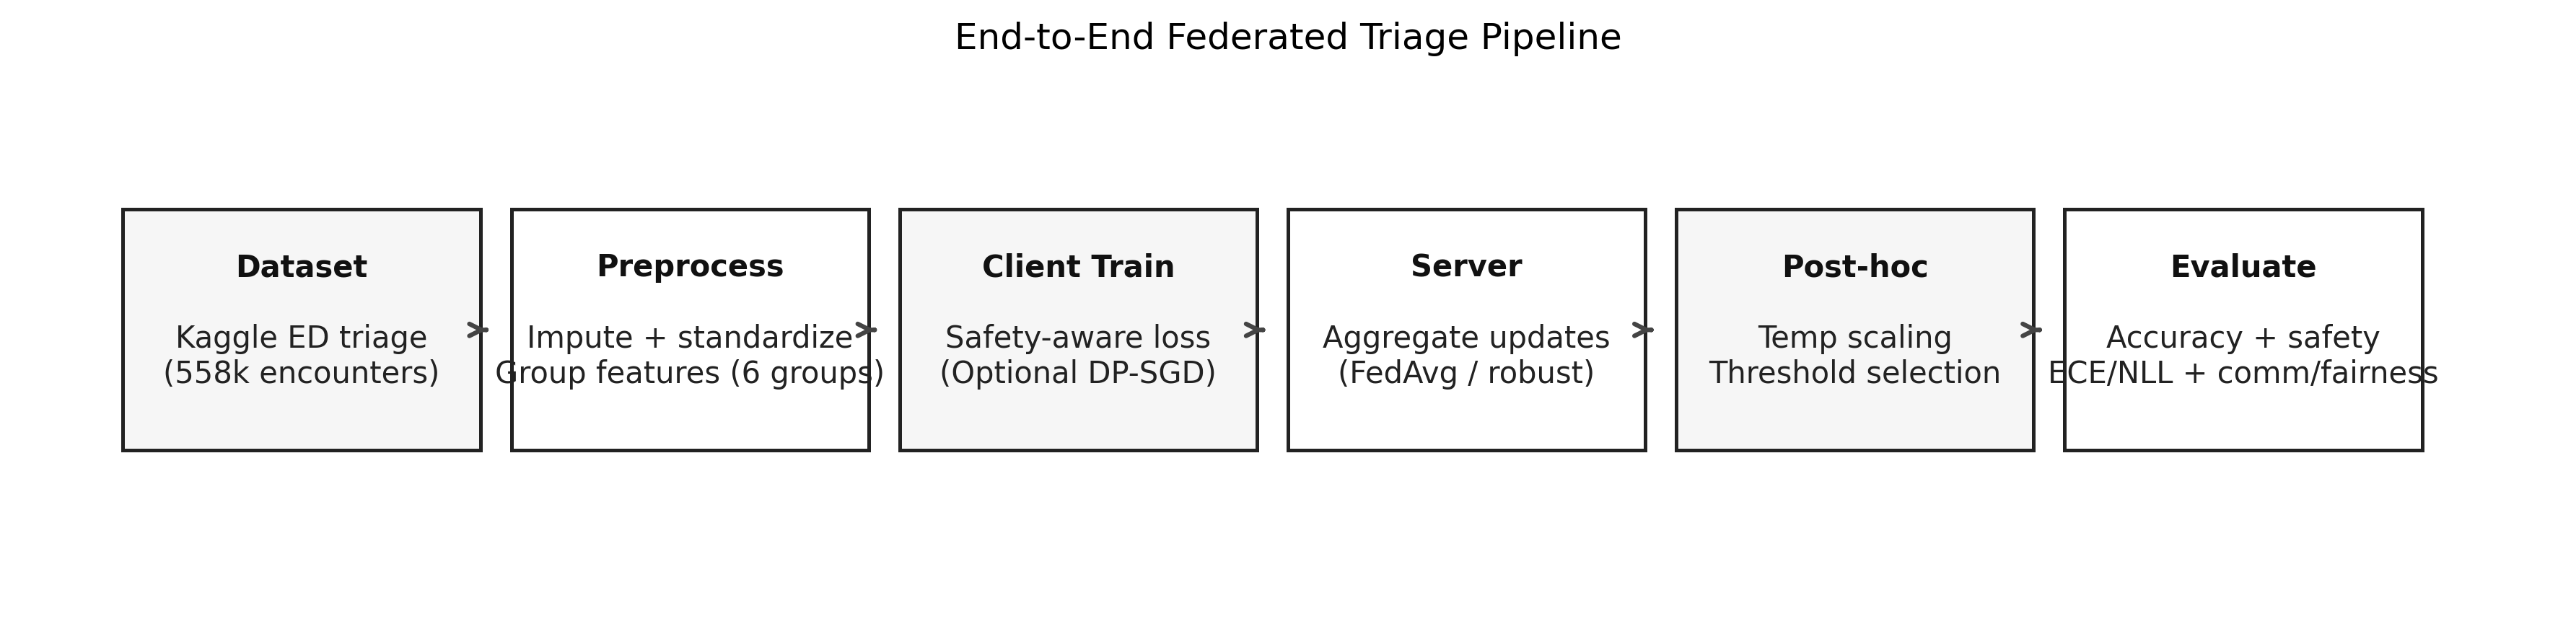
\includegraphics[width=\textwidth]{figures/pipeline_overview.png}
\caption{End-to-end federated triage pipeline used in this study: preprocessing and feature grouping, client-side safety-aware training (optionally with DP-SGD), server aggregation, post-hoc calibration/thresholding, and evaluation across utility, safety, reliability, and communication.}
\label{fig:pipeline-overview}
\end{figure}

%%%%%%%%%%%%%%%%%%%%%%%%%%%%%%%%%%%%%%%%%%
\section{Experiments}\label{sec:experiments}

\subsection{Evaluation Metrics}

We evaluate our models using a comprehensive set of metrics that cover classification performance, clinical safety, calibration, privacy, fairness, and efficiency. For classification performance, we report overall accuracy, per-class precision, recall, F1-score, and macro-averaged F1-score. To quantify uncertainty, we compute bootstrap 95\% confidence intervals using 1000 resamples. Clinical safety is assessed using three key metrics: critical sensitivity, which is the recall for the critical band (ESI-2, ESI-1); the under-triage rate, defined as the fraction of predictions where the predicted severity is lower than the ground truth; and the over-triage rate, the fraction of predictions where the predicted severity is higher than the ground truth. To evaluate model calibration and reliability, we measure the negative log-likelihood (NLL), the expected calibration error (ECE) with 10 bins, and the Brier score \cite{guo2017}. We also generate reliability diagrams to visualize the correspondence between predicted probabilities and observed frequencies. The privacy–utility trade-off is quantified by the privacy budget $(\varepsilon, \delta)$ per round in federated settings or per epoch in centralized training. We also plot validation accuracy against $\varepsilon$ to create privacy–utility curves for our differential privacy experiments. To support fairness-aware deployment, we report subgroup metrics across gender and age groups and flag large subgroup disparities (max--min differences above 0.1 on selected metrics) as descriptive diagnostics. Interpretability is addressed through SHAP global feature importance and class-conditional attributions. Finally, we measure communication and efficiency by tracking the per-round communication in bytes uploaded and downloaded per client, the per-round wall-clock time and its variance across clients, the model size, and the inference latency.

\subsection{Baselines and Configurations}

We compare our proposed model against several baselines and configurations. The centralized neural baseline is trained on the full training split with validation-based checkpoint selection and post-hoc operating-point selection. For cross-silo FL, we use a site-aligned partition using the dataset's hospital-department identifier as a proxy for three real sites. We run 20 communication rounds with three clients and one local epoch per round (FedAvg). The flat FL baseline trains the single-head model, while the red-focus hierarchical variant uses a gate + specialist-head structure and safety-aware loss shaping to emphasize the critical band. We include a differentially private ablation (DP-SGD; 3 sites; 5 rounds; $\sigma=1.0$, $\delta=10^{-5}$; Adam) to illustrate privacy--utility trade-offs under client-side DP. To ground performance, we also evaluate a strong traditional tabular baseline (HistGradientBoosting). Finally, to empirically validate robust aggregation, we run a Byzantine simulation in a non-IID setting (7 clients, Dirichlet $\alpha=0.3$, 10 rounds) and compare FedAvg to coordinate-wise median under a Gaussian poisoning attack (29\% malicious clients per round).

\subsection{Hyperparameters}

We use a fixed random seed of 42 for reproducibility. Unless otherwise stated, the optimizer is Adam with default betas and gradient clipping with a norm of 1.0. Centralized training uses a batch size of 256 and a learning rate of $5\times 10^{-3}$ for 10 epochs, with dropout rates from 0.1 to 0.4 depending on the block. In cross-silo FL (site-aligned, 3 clients), we run 20 rounds with 1 local epoch per round, batch size 256, and learning rate $5\times 10^{-3}$ (FedAvg). For the Byzantine robustness evaluation (7 clients, Dirichlet $\alpha=0.3$), we use 10 rounds with 1 local epoch per round, batch size 256, and learning rate $5\times 10^{-3}$; under attack, 29\% of clients are corrupted each round via a Gaussian perturbation applied to their parameter updates. Temperature scaling is selected on the validation set by minimizing NLL (via a small grid search). When differential privacy is enabled, we use DP-SGD via Opacus with $\sigma=1.0$, $\delta=10^{-5}$, an Adam optimizer on each client, and composed $(\varepsilon,\delta)$ accounting across rounds.

For traceability, all main ESI-5 figures and tables in this manuscript were regenerated from the latest report artifacts produced by the released scripts: centralized (\texttt{advanced\_evaluation\_report\_20260210\_140144.json}), cross-silo FL flat (\texttt{fl\_advanced\_evaluation\_report\_20260211\_105235.json}), cross-silo FL red-focus (\texttt{fl\_advanced\_red\_focus\_evaluation\_report\_20260211\_110907.json}), DP-SGD (\texttt{fl\_advanced\_evaluation\_report\_20260211\_103558.json}), and Byzantine runs (\texttt{fl\_advanced\_evaluation\_report\_20260211\_111723.json}, \texttt{fl\_advanced\_evaluation\_report\_20260211\_112534.json}, \texttt{fl\_advanced\_evaluation\_report\_20260211\_113403.json}). Figures are generated by \texttt{scripts/generate\_paper\_figures.py} and validated by \texttt{scripts/audit\_paper\_artifacts.py}.

%%%%%%%%%%%%%%%%%%%%%%%%%%%%%%%%%%%%%%%%%%
\section{Results}\label{sec:results}

\subsection{Operational 3-Class Triage (ESI Binning)}

Because ESI-1 and ESI-5 are rare, we additionally evaluate a 3-class operational mapping derived from ESI: Green (ESI-5/ESI-4), Yellow (ESI-3), and Red (ESI-2/ESI-1). This binning is clinically interpretable (low/medium/high acuity) and reduces extreme-class sparsity, which stabilizes macro-averaged metrics. Table~\ref{tab:3class} shows that, in this coarse setting, federated learning can remain close to centralized training: a small 2-client, 2-round flat FL baseline reaches 86.6\% accuracy and the red-focus variant reaches 87.0\% accuracy with Red recall 0.846, compared to 88.9\% accuracy and Red recall 0.869 for the centralized model. We treat these 3-class results as an operational sanity-check; the remainder of the paper focuses on the full ESI-5 task, where extreme-class failures and safety trade-offs are more pronounced.

\begin{table}[H]
\centering
\caption{Operational 3-class triage results (Green/Yellow/Red; derived from ESI). Red recall corresponds to critical sensitivity in the binned setting.}
\label{tab:3class}
\small
\begin{tabular}{lccccc}
\toprule
System & Acc & Weighted-F1 & Macro-F1 & Red Recall & Under-Triage \\
\midrule
Centralized (non-DP) & 0.889 & 0.889 & 0.890 & 0.869 & 0.040 \\
FL Flat (non-DP; 2 clients, 2 rounds) & 0.866 & 0.867 & 0.868 & 0.808 & 0.058 \\
FL Red-Focus (non-DP; 2 clients, 2 rounds) & 0.870 & 0.871 & 0.872 & 0.846 & 0.072 \\
\bottomrule
\end{tabular}
\end{table}

Figure~\ref{fig:confusion-matrices-3class} shows the corresponding confusion matrices. In this binned setting, both centralized and federated models preserve a strong diagonal structure, and most errors occur between adjacent acuity bands.

\begin{figure}[H]
\centering
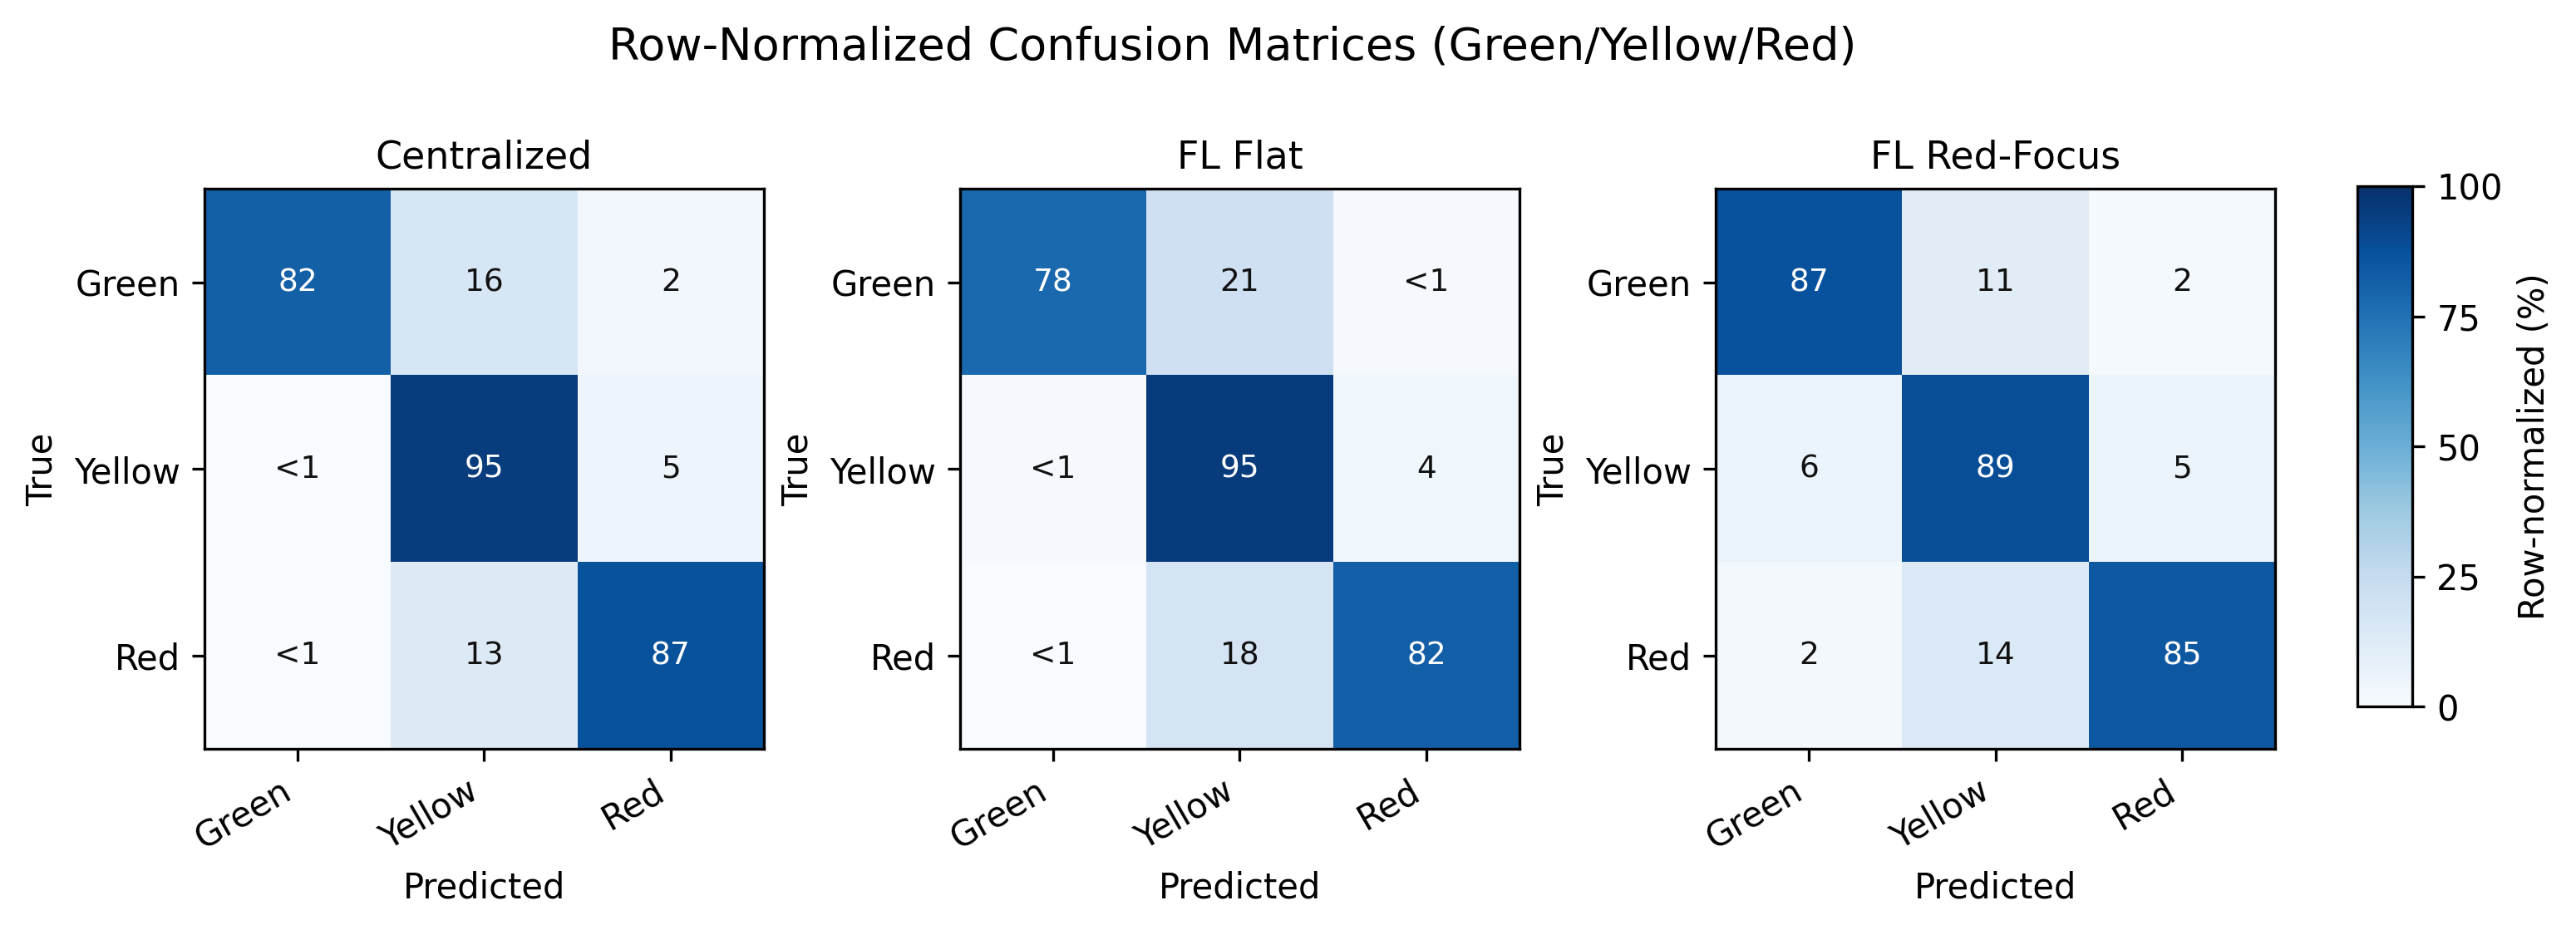
\includegraphics[width=\textwidth]{figures/confusion_matrices_3class.png}
\caption{Row-normalized confusion matrices (Green/Yellow/Red). The federated models remain close to the centralized baseline on this coarser operational decision, with errors concentrated between adjacent classes.}
\label{fig:confusion-matrices-3class}
\end{figure}

\subsection{ESI-5: Centralized vs Federated Performance}

Table~\ref{tab:core-metrics} summarizes test-set performance and safety metrics on ESI-5 across centralized and federated configurations. We include a strong non-neural tabular baseline (HistGradientBoosting) alongside our attention model. The centralized neural model reaches 85.4\% accuracy and 95.3\% critical-band sensitivity at a safety-oriented operating point (C$^3$ on validation). In cross-silo FL using three real sites (hospital departments), a flat FedAvg baseline (20 rounds) achieves 75.3\% accuracy and 80.2\% critical sensitivity, while the red-focus hierarchical variant improves to 80.5\% accuracy and 90.8\% critical sensitivity. For these federated models, our strict validation-time safety constraints were infeasible at this training horizon, so the reported FL metrics correspond to temperature-scaled argmax decisions rather than a constrained operating-point solution. Macro-F1 remains sensitive to extreme classes and operating-point choices; in our DP-SGD run, accuracy remains high (0.843) at $\varepsilon\approx1.15$, but ESI-1 recall is 0.0, which reduces macro-F1 (0.683) and critical sensitivity (0.781).

\begin{table}[H]
\centering
\caption{Test-set performance and safety metrics (ESI-5). Critical sensitivity is recall for the top-2 severity classes (ESI-2/ESI-1).}
\label{tab:core-metrics}
\small
\begin{tabular}{lccccc}
\toprule
System & Acc & Weighted-F1 & Macro-F1 & Crit.\ Sens. & Under-Triage \\
\midrule
HistGB (centralized) & 0.895 & 0.895 & 0.915 & 0.885 & 0.036 \\
Centralized NN (non-DP) & 0.854 & 0.856 & 0.872 & 0.953 & 0.015 \\
FL Flat (non-DP; 3 sites, 20 rounds) & 0.753 & 0.812 & 0.672 & 0.802 & 0.217 \\
FL Red-Focus (non-DP; 3 sites, 20 rounds) & 0.805 & 0.830 & 0.777 & 0.908 & 0.133 \\
DP-SGD (3 sites, 5 rounds; $\sigma=1.0$; Adam) & 0.843 & 0.839 & 0.683 & 0.781 & 0.075 \\
\bottomrule
\end{tabular}
\end{table}

\noindent\textbf{Uncertainty and effect sizes.} We compute bootstrap 95\% confidence intervals (1000 resamples) for the core metrics. The red-focus FL variant improves accuracy by +5.2 points over flat FL (0.805 vs.\ 0.753; CIs do not overlap) and improves critical sensitivity by +10.6 points (0.908 vs.\ 0.802), while reducing under-triage by 8.4 points (0.133 vs.\ 0.217). These gaps are large relative to the bootstrap uncertainty, indicating that the red-focus improvement is not a sampling artifact on the held-out test set.

\begin{figure}[H]
\centering
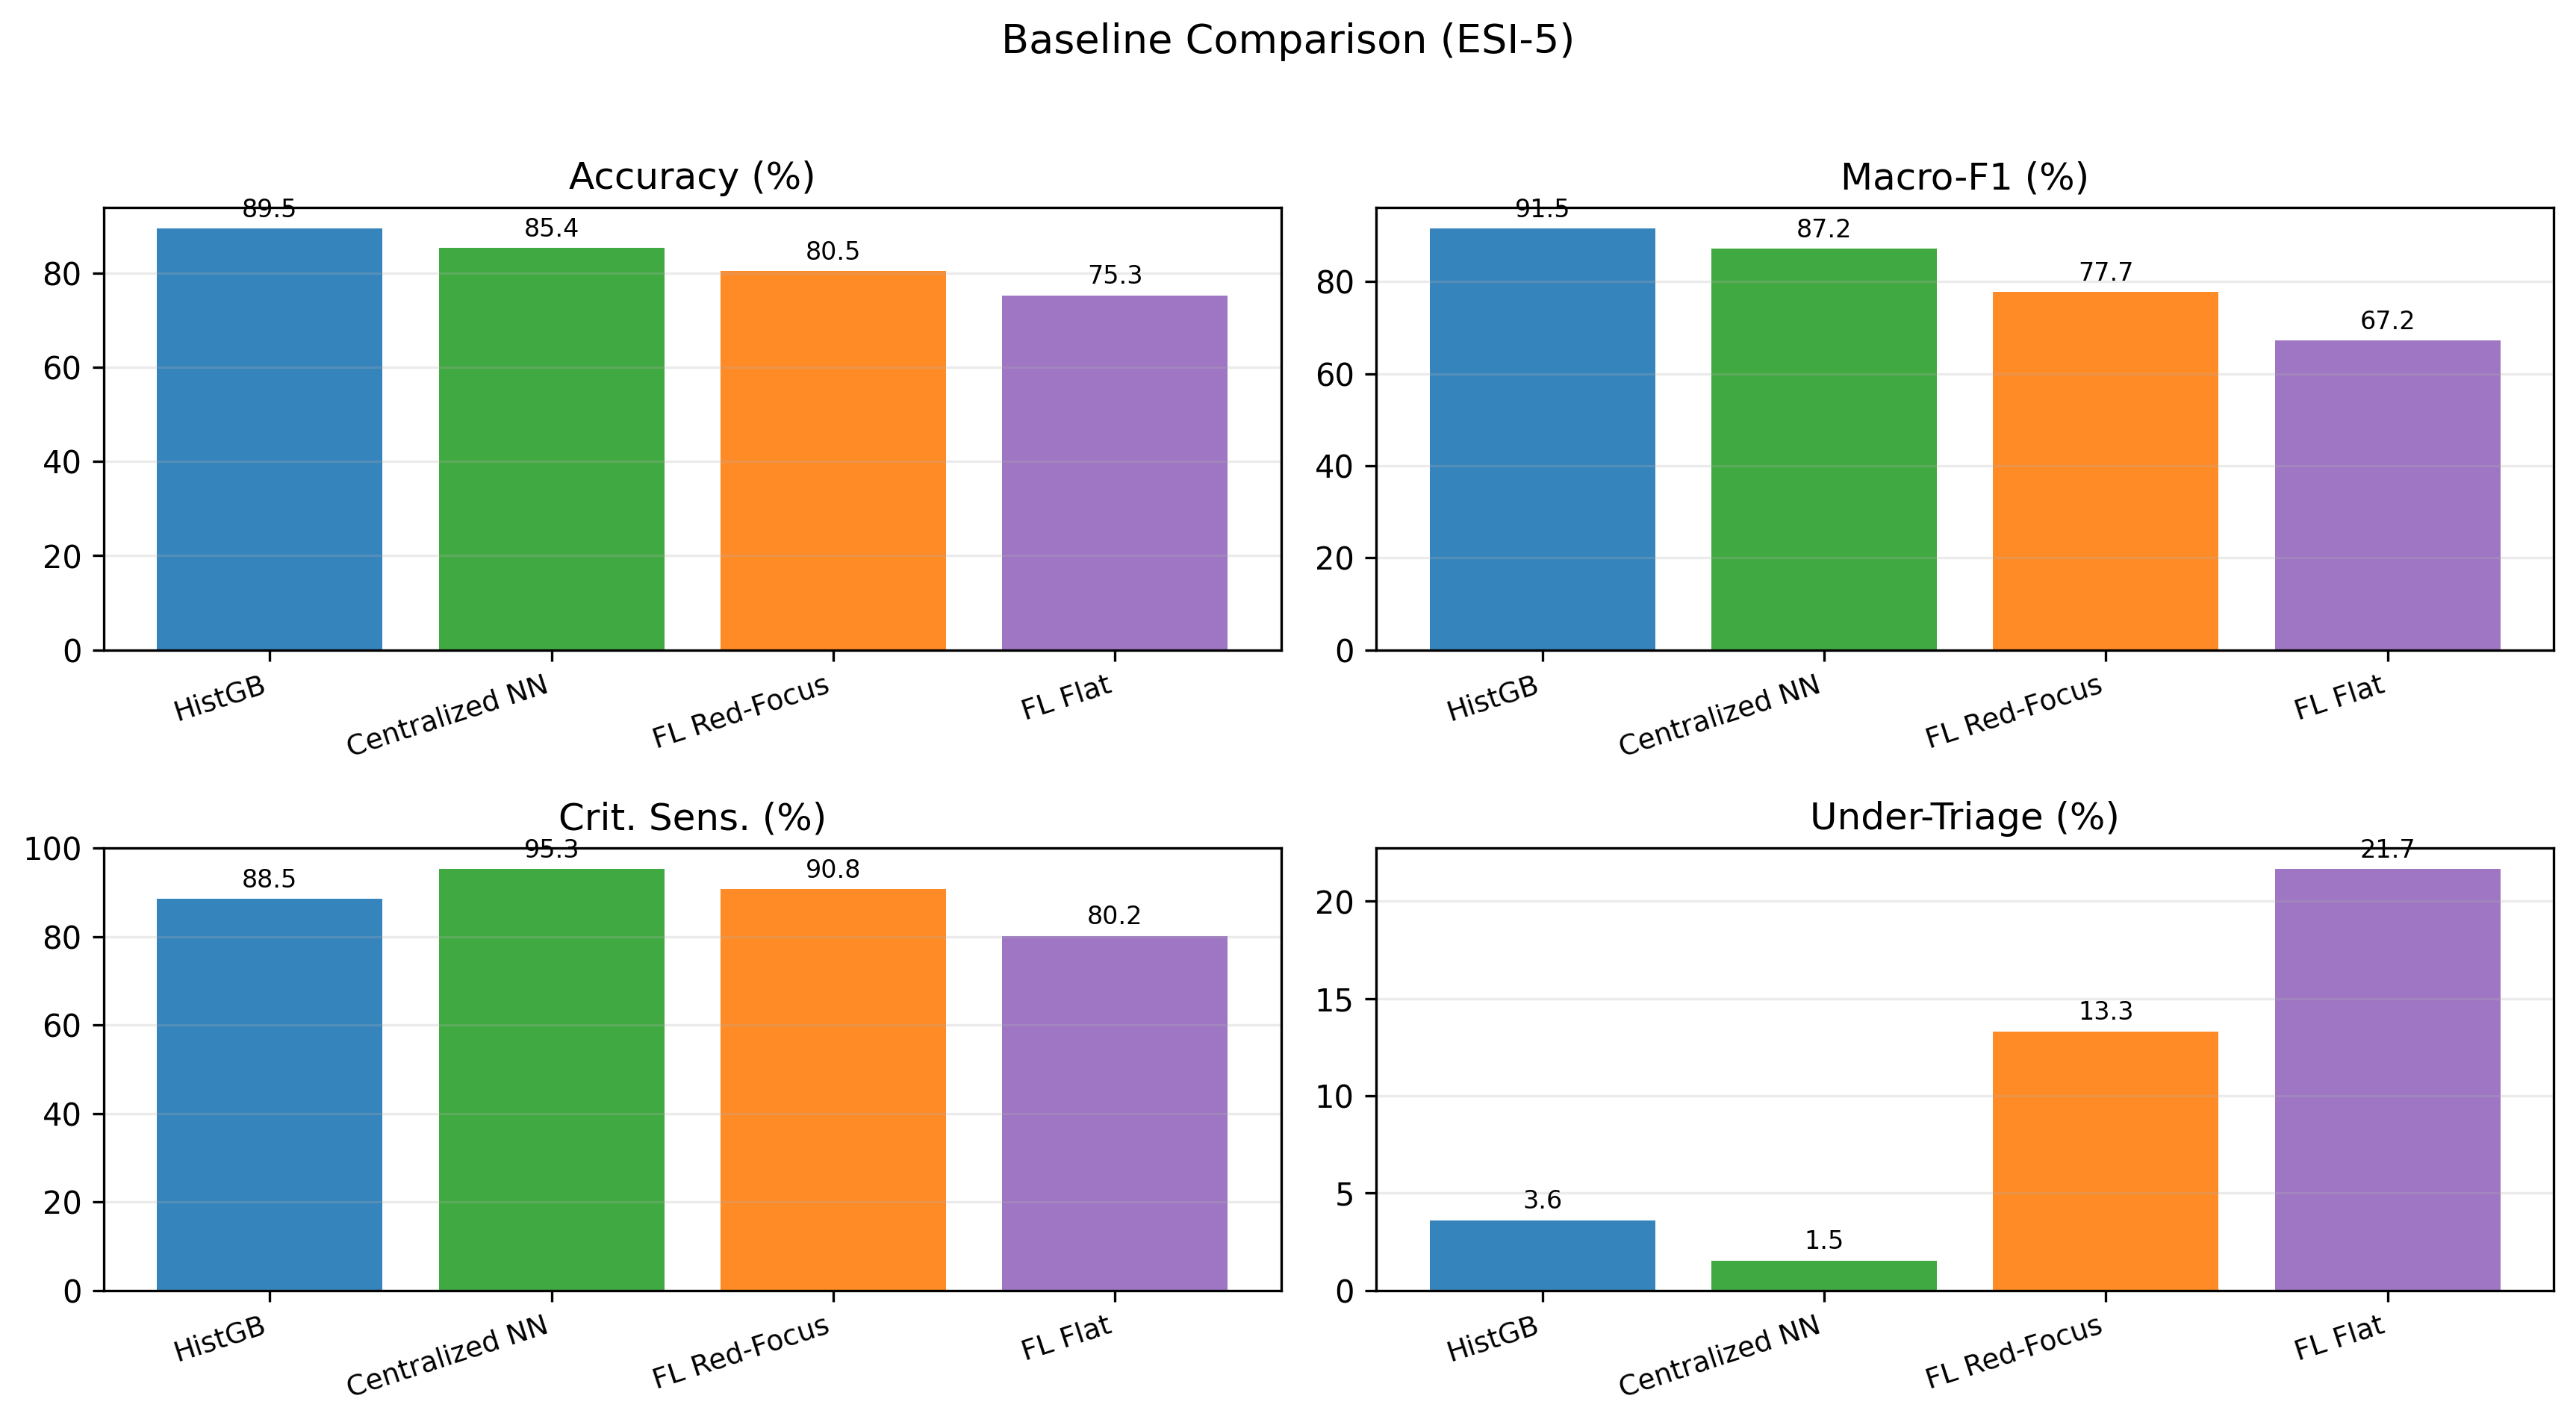
\includegraphics[width=\textwidth]{figures/baseline_comparison.png}
\caption{Baseline comparison on ESI-5. The HistGradientBoosting (HistGB) baseline provides a strong non-neural reference, while the red-focus FL model improves safety metrics relative to the flat FL baseline.}
\label{fig:baseline-comparison}
\end{figure}

Although the federated red-focus model remains below the strongest centralized baselines in overall accuracy, it achieves competitive safety metrics without pooling data, which avoids direct data sharing and reduces regulatory friction. The remaining gap can likely be narrowed by increasing communication rounds, adding personalization, and improving client-side optimization under heterogeneous (non-IID) client distributions.

\begin{figure}[H]
\centering
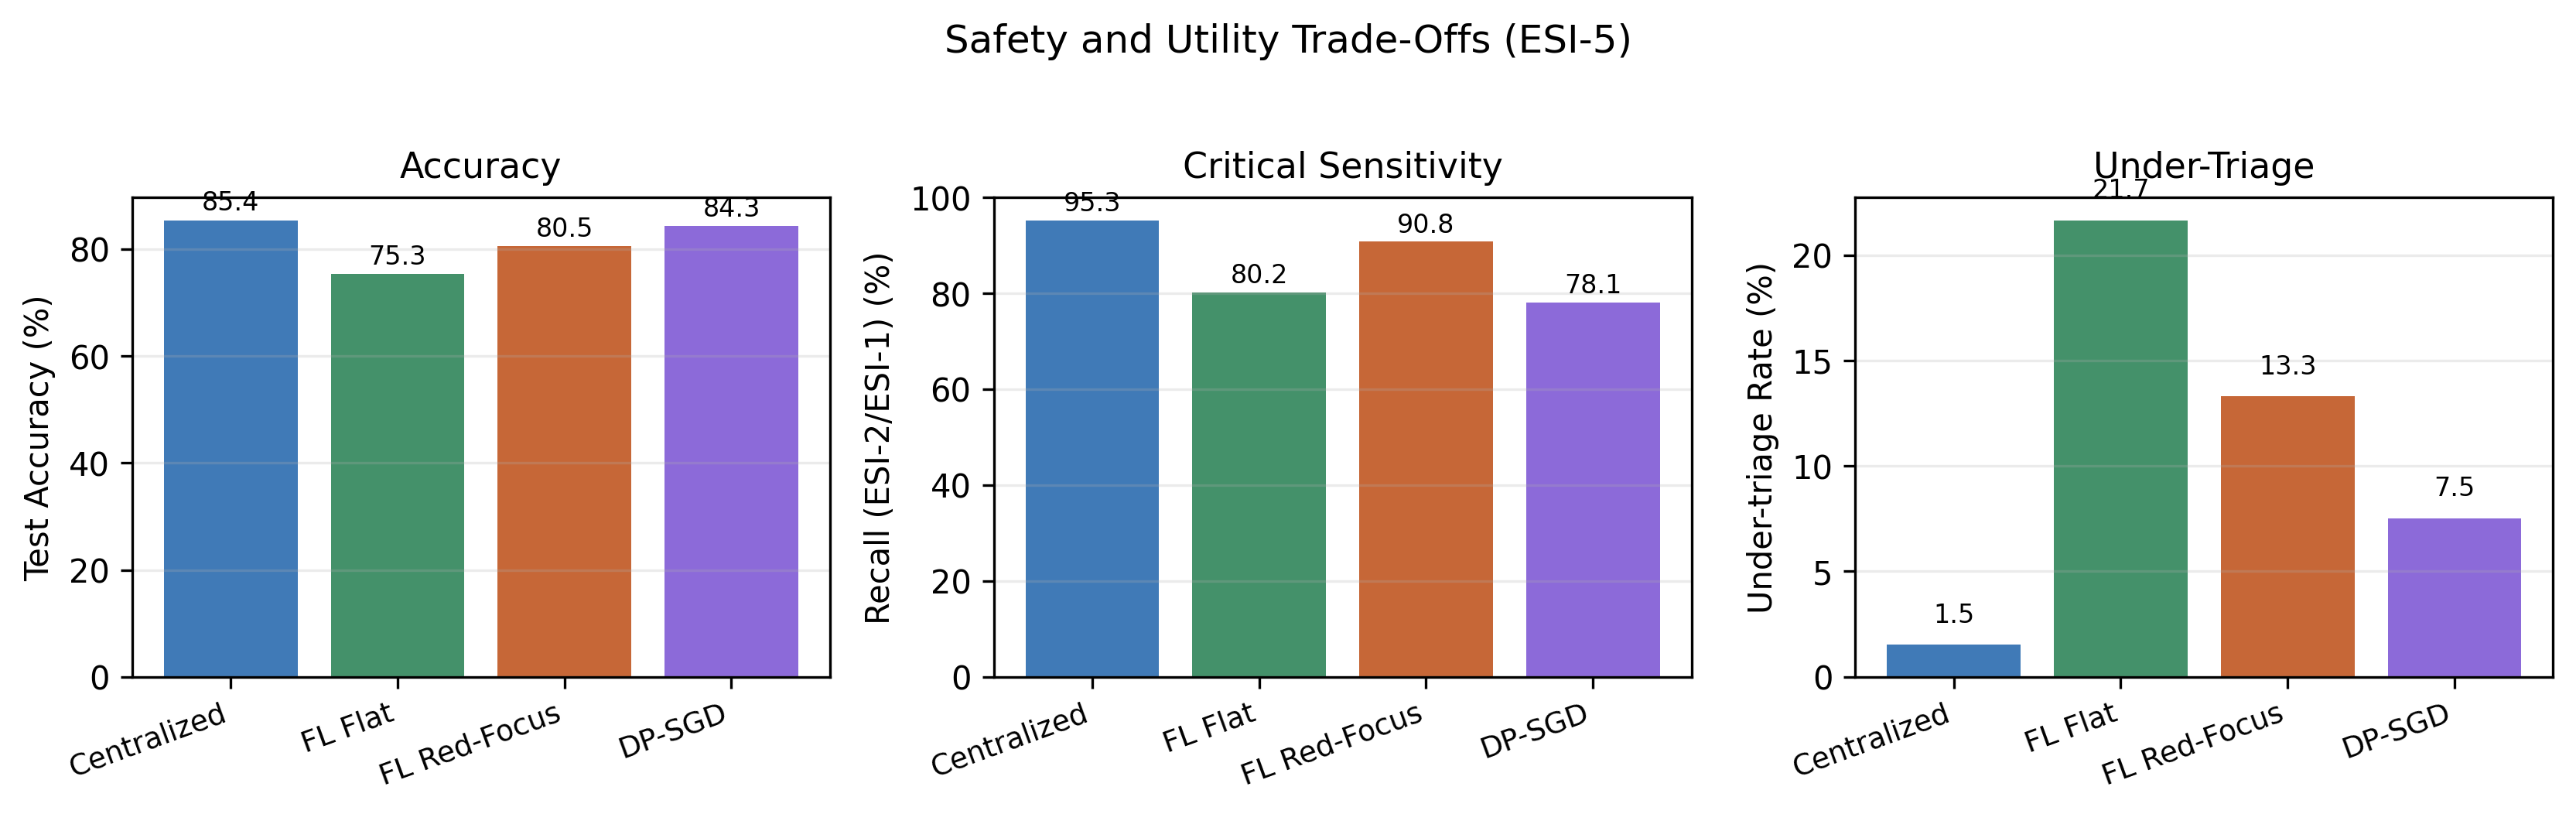
\includegraphics[width=\textwidth]{figures/safety_tradeoff.png}
\caption{Safety and utility trade-offs on ESI-5 across the core configurations. The red-focus hierarchical FL variant improves safety relative to the flat FL baseline (higher critical sensitivity; lower under-triage) while maintaining extreme-class recall in the non-DP setting. DP-SGD provides formal privacy ($\varepsilon\approx1.15$) but substantially degrades extreme-class performance (ESI-1 recall 0.0), which depresses macro-F1 and critical sensitivity despite high overall accuracy.}
\label{fig:safety-tradeoff}
\end{figure}

\subsection{Clinical Safety Metrics}

Table~\ref{tab:safety} focuses on safety for the critical band and the rare extreme classes. In the non-DP runs, both cross-silo FL variants maintain high recall for ESI-1 and ESI-5 while the red-focus model substantially improves critical sensitivity and reduces under-triage compared to the flat baseline. In contrast, DP-SGD maintains high overall accuracy but fails to predict ESI-1 (0.0 recall), reducing macro-F1 and critical sensitivity relative to non-DP baselines.

\begin{table}[H]
\centering
\caption{Clinical safety diagnostics (ESI-5). Critical sensitivity is recall for the critical band (ESI-2/ESI-1).}
\label{tab:safety}
\small
\begin{tabular}{lcccc}
\toprule
System & ESI-1 Recall & ESI-5 Recall & Critical Sensitivity & Under-Triage Rate \\
\midrule
HistGB (centralized) & 0.943 & 0.878 & 0.885 & 0.036 \\
Centralized NN (non-DP) & 0.956 & 0.862 & 0.953 & 0.015 \\
FL Flat (non-DP; 3 sites, 20 rounds) & 0.973 & 0.994 & 0.802 & 0.217 \\
FL Red-Focus (non-DP; 3 sites, 20 rounds) & 0.964 & 0.963 & 0.908 & 0.133 \\
DP-SGD (3 sites, 5 rounds; $\sigma=1.0$; Adam) & 0.000 & 0.782 & 0.781 & 0.075 \\
\bottomrule
\end{tabular}
\end{table}

High critical sensitivity means the model rarely misses patients who need immediate attention, which is an essential safety requirement in ED triage. In our cross-silo setting, the red-focus hierarchical approach improves critical sensitivity relative to the flat FL baseline (0.908 vs.\ 0.802) and reduces under-triage (0.133 vs.\ 0.217), moving closer to the centralized neural operating point (0.953 critical sensitivity; 0.015 under-triage). Notably, both non-DP federated models maintain high ESI-1 recall ($\geq$0.964), and the critical-sensitivity gap is driven primarily by ESI-2 recall (0.757 for flat FL vs.\ 0.899 for red-focus FL), consistent with the intended design of prioritizing the critical band while preserving extreme-class detection.

\begin{figure}[H]
\centering
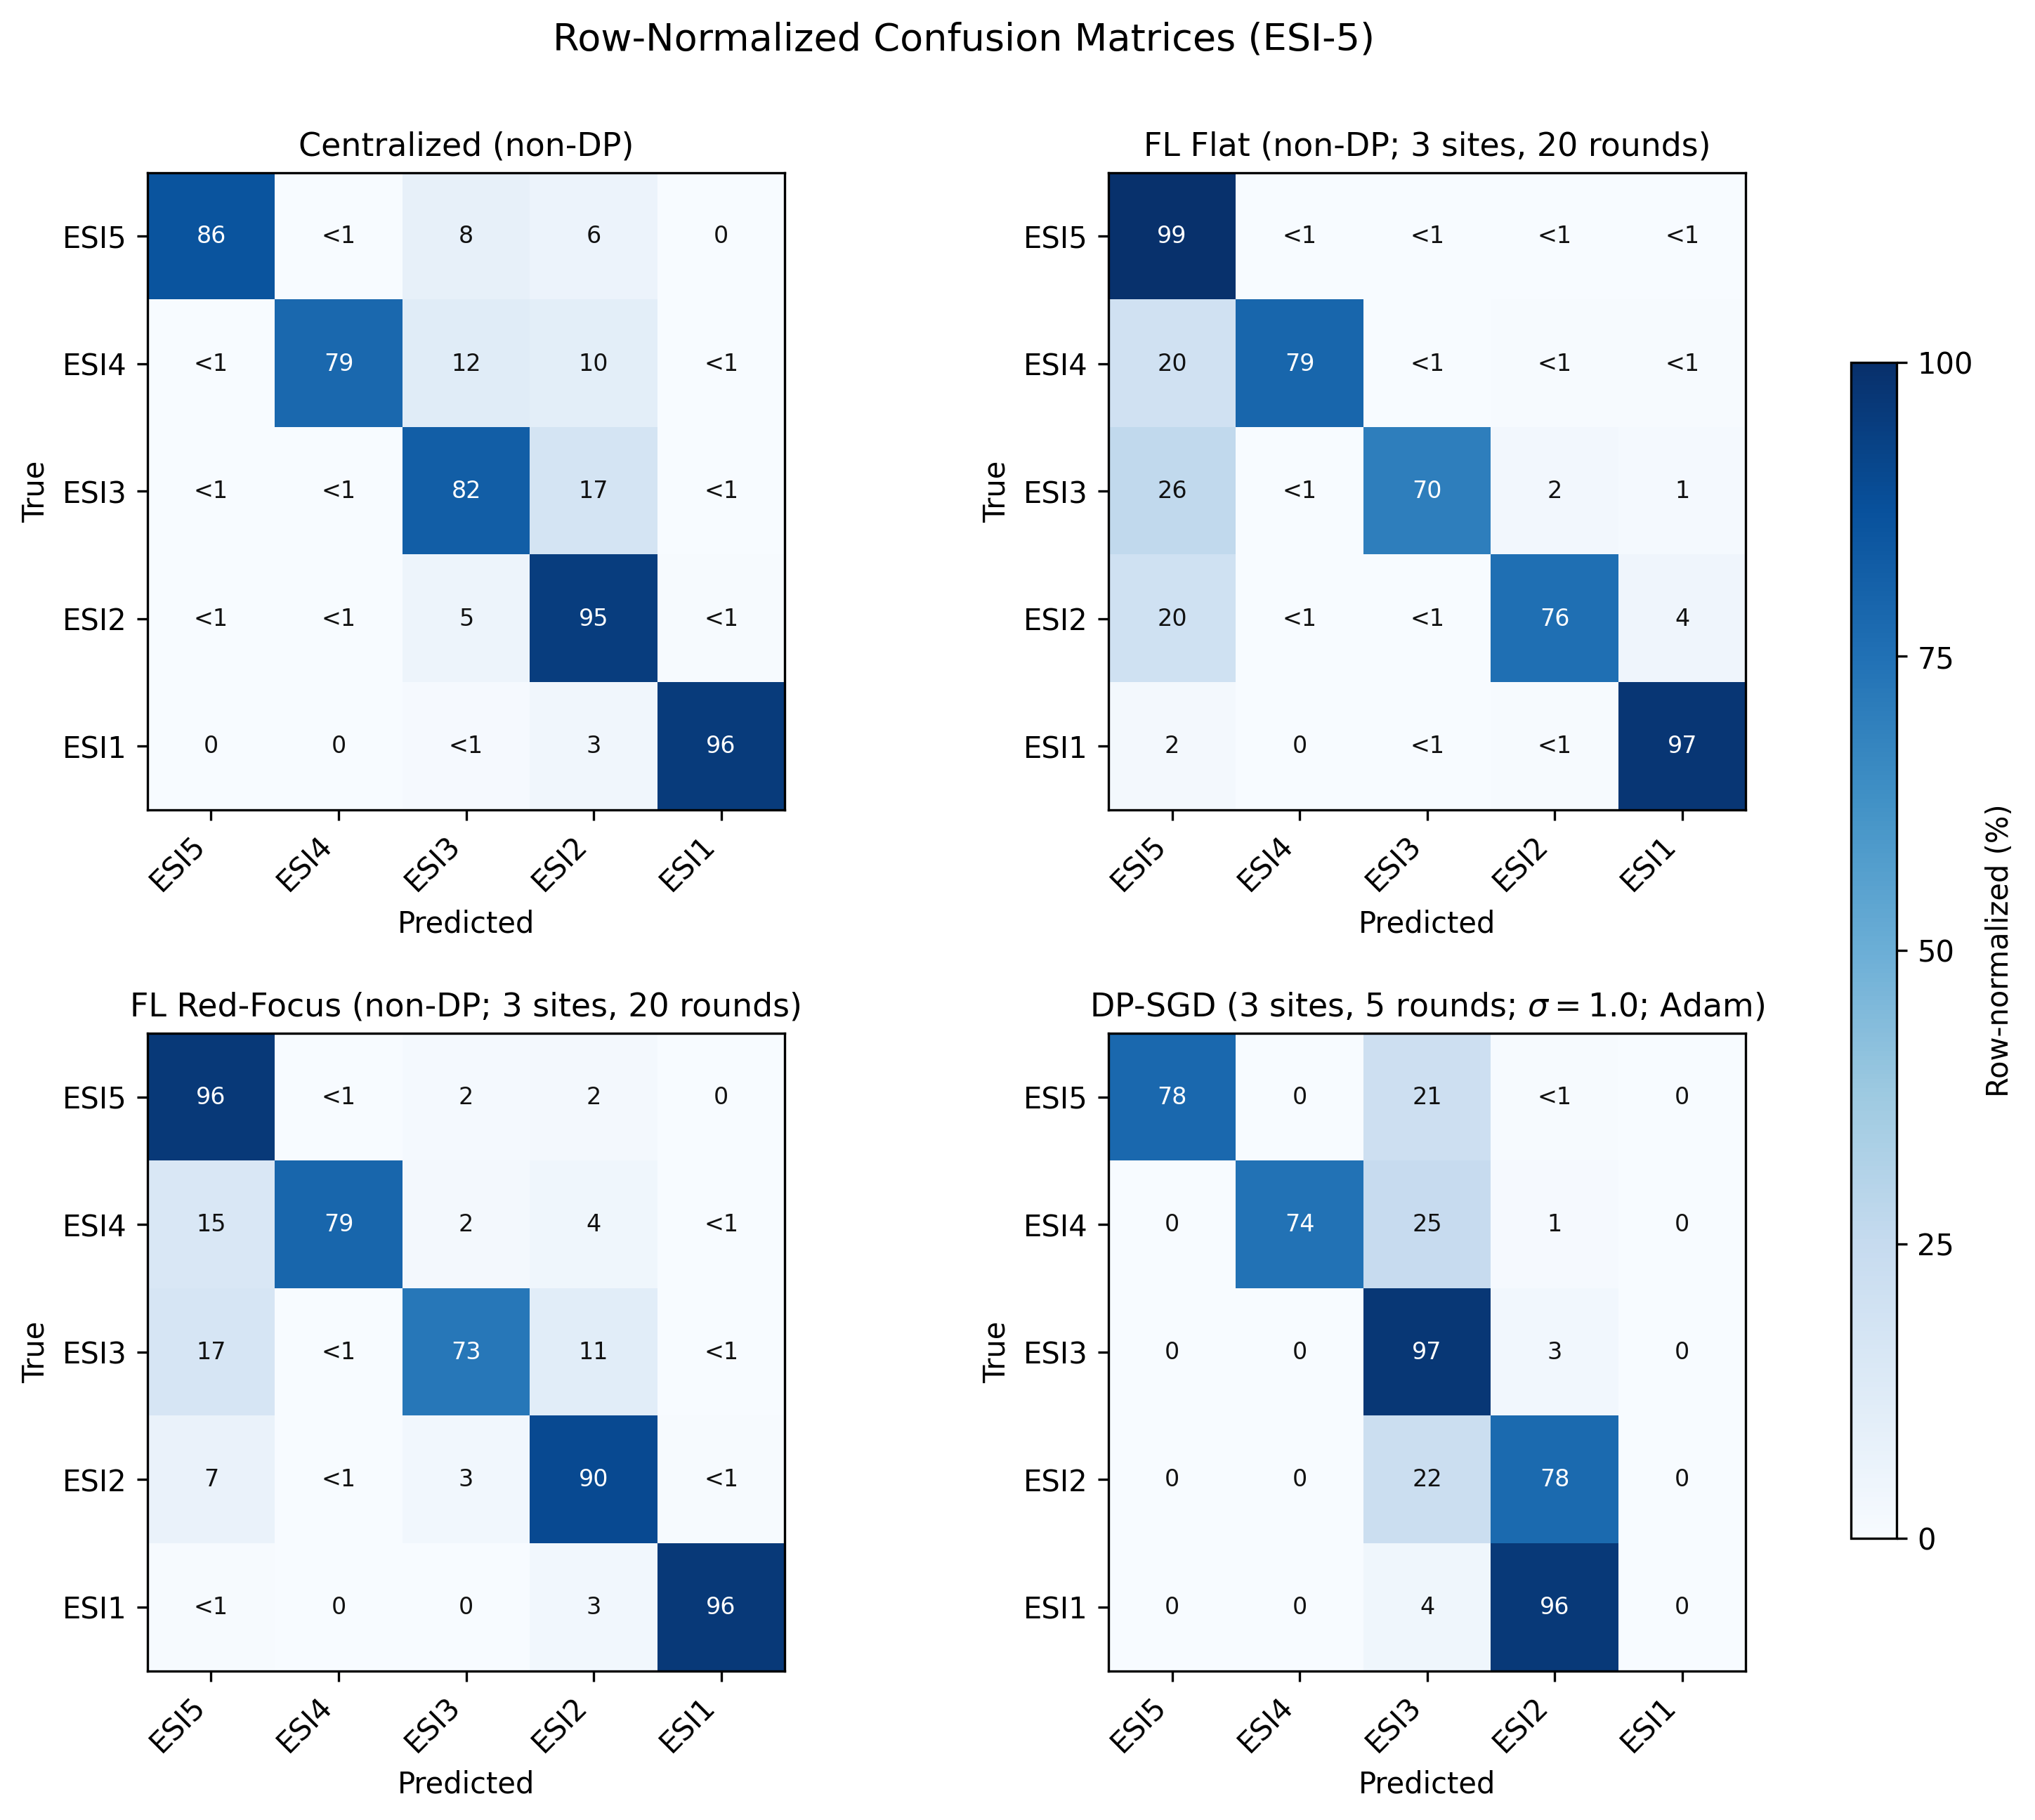
\includegraphics[width=\textwidth]{figures/confusion_matrices_esi5.png}
\caption{Row-normalized confusion matrices (ESI-5). In cross-silo FL, the flat FedAvg baseline shows substantial under-triage from ESI-3 toward lower acuity, while the red-focus hierarchical variant improves critical-band discrimination. The DP-SGD run fails to predict ESI-1 (0.0 recall) and concentrates predictions in the mid-acuity classes, which reduces macro-F1 and critical sensitivity despite high overall accuracy.}
\label{fig:confusion-matrices}
\end{figure}

\subsection{Privacy-Utility Trade-Off with Differential Privacy}

Figure~\ref{fig:privacy-utility} summarizes privacy accounting and utility for a DP-SGD cross-silo run (3 sites, 5 rounds; $\sigma=1.0$, $\delta=10^{-5}$). We compute a composed privacy budget using R\'enyi DP accounting and track the maximum client privacy loss across rounds.

In this run, the composed privacy budget reaches $\varepsilon\approx1.15$ (max client), and validation accuracy rises from 80.0\% in Round~1 to $\sim$84\% by Round~2--5. However, accuracy alone is misleading in this imbalanced setting: because ESI-1 constitutes only 0.9\% of encounters, a model can achieve high overall accuracy while still failing on the rarest (and most safety-critical) class. On the held-out test set, the DP-SGD model predicts no ESI-1 cases (0.0 recall and 0.0 precision), mapping true ESI-1 examples into mid-acuity classes; consequently, macro-F1 drops to 0.683 and critical sensitivity drops to 0.781 despite 0.843 overall accuracy.

\begin{table}[H]
\centering
\caption{DP run (3 sites, 5 rounds; $\sigma=1.0$, $\delta=10^{-5}$): composed privacy budget (max client) and validation accuracy.}
\label{tab:dp-eps-acc}
\small
\begin{tabular}{lcc}
\toprule
Round & $\varepsilon$ (composed; max client) & Val Acc (\%) \\
\midrule
1 & 0.938 & 80.0 \\
2 & 0.999 & 84.6 \\
3 & 1.053 & 84.3 \\
4 & 1.104 & 84.3 \\
5 & 1.153 & 84.2 \\
\bottomrule
\end{tabular}
\end{table}
We report the maximum composed $\varepsilon$ across clients after each round using R\'enyi DP accounting (fixed $\delta=10^{-5}$).

\begin{figure}[H]
\centering
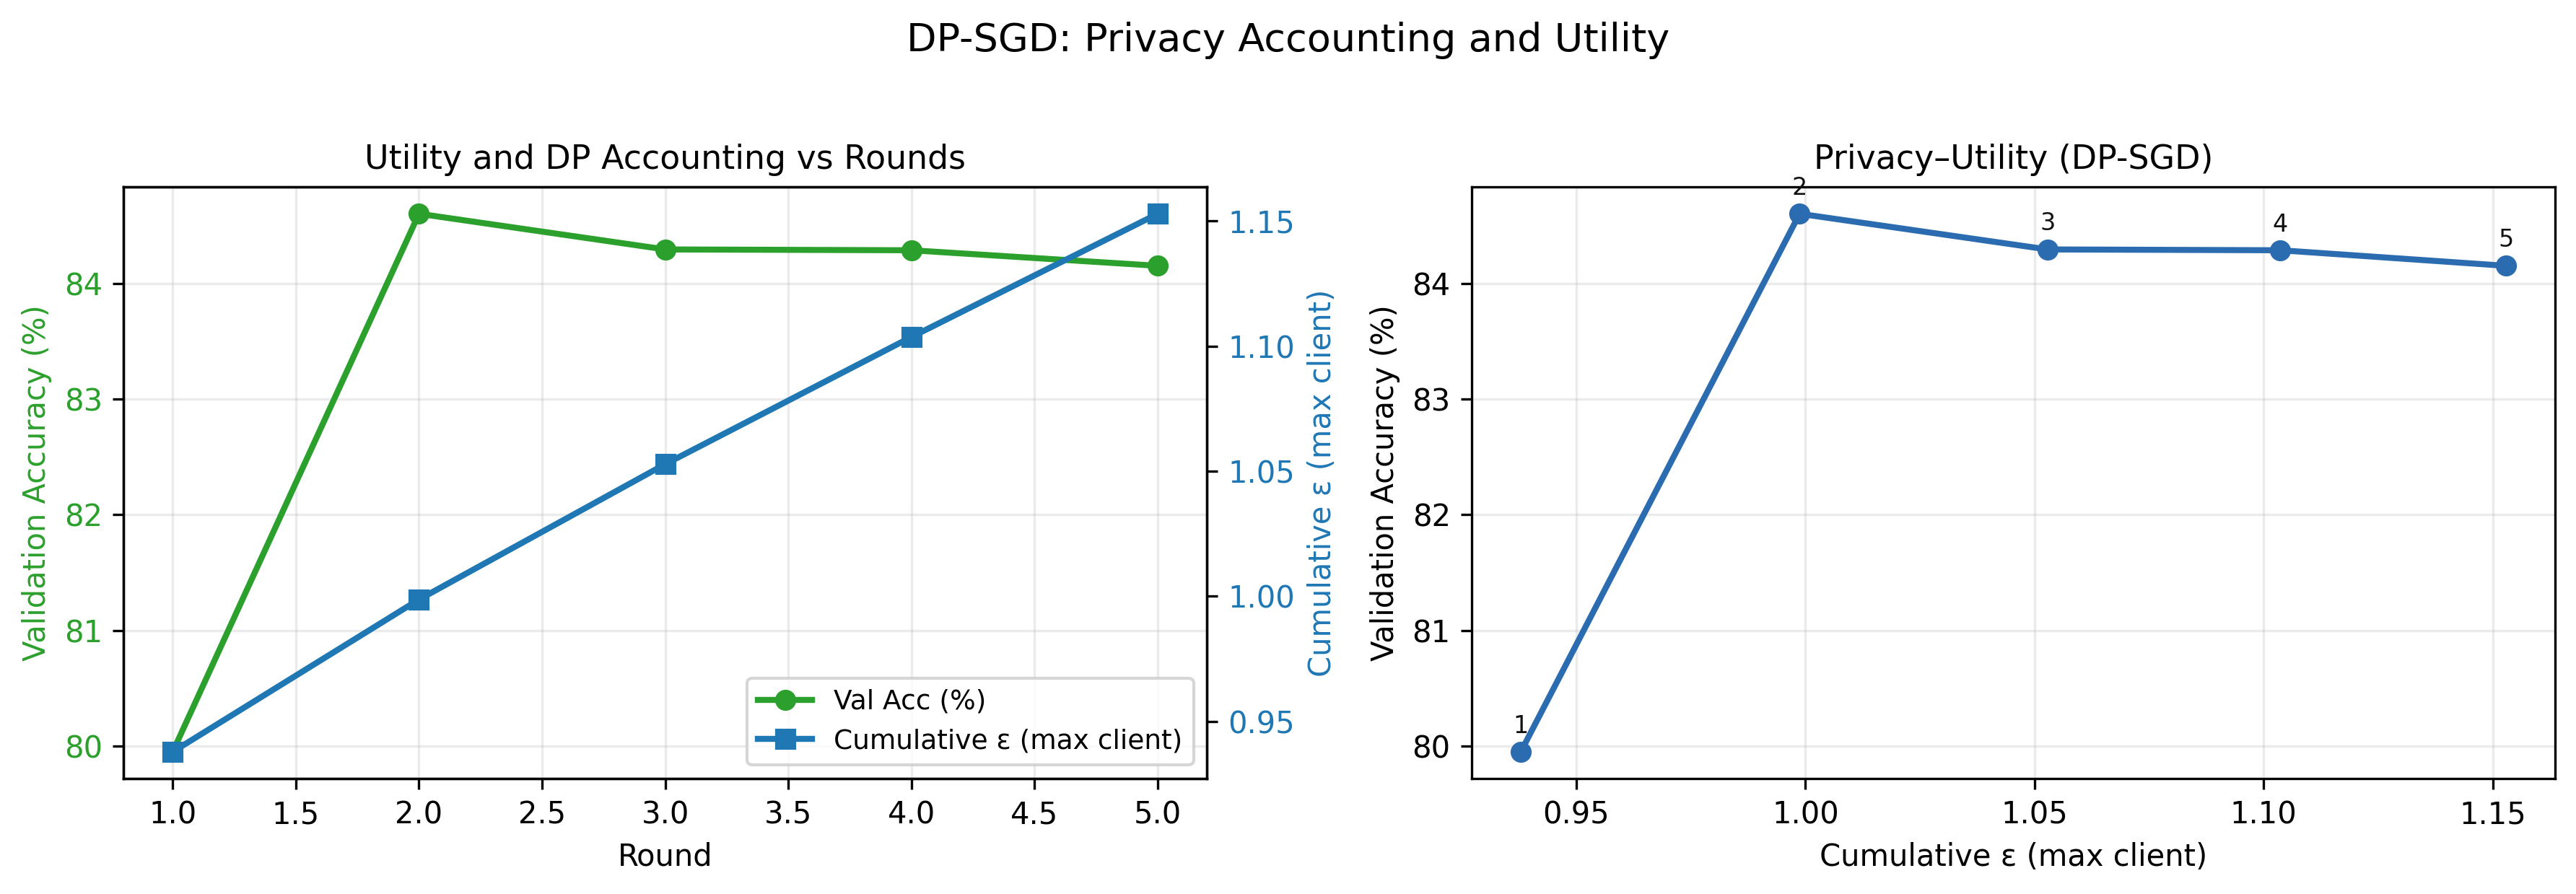
\includegraphics[width=0.8\textwidth]{figures/fl_advanced_privacy_utility.png}
\caption{DP-SGD privacy accounting and utility (3 sites, 5 rounds; $\sigma=1.0$; $\delta=10^{-5}$). Left: validation accuracy and composed privacy budget $\varepsilon$ (max client) across rounds. Right: a privacy--utility view using the composed $\varepsilon$ on the x-axis. Validation accuracy reaches $\sim$84\% by Round~2--5 at $\varepsilon\approx1.15$, but the DP model fails to predict ESI-1 (0.0 recall), highlighting that accuracy alone can mask extreme-class failures under DP.}
\label{fig:privacy-utility}
\end{figure}

The DP run remains competitive in overall accuracy but is not clinically reliable for the rarest acuity level (ESI-1), where recall is 0.0 on the test set. Improving this frontier likely requires more communication rounds and DP-specific optimization techniques (e.g., clipping/noise tuning, per-layer clipping, and privacy-aware hyperparameter searches), as well as objectives that explicitly stabilize minority-class learning under gradient clipping.

DP-SGD mitigates gradient inversion and membership inference by clipping per-sample gradients and adding calibrated noise. These protections come with substantial costs for rare-class learning in our multi-class triage setting, as reflected in the extreme-class recall degradation observed in the DP ablation.

\subsection{Robust Aggregation for Byzantine Resilience}

We evaluate robust aggregation under a simulated Byzantine threat. In a non-IID setting (7 clients, Dirichlet $\alpha=0.3$, 10 rounds), we corrupt 29\% of clients per round using a Gaussian attack on the model updates. Under this attack, FedAvg accuracy drops to 61.4\% and over-triage increases to 36.8\%. Notably, FedAvg critical sensitivity increases to 0.970 under attack because the model over-triages many cases into the critical band; this is a safety-inefficient failure mode rather than a clinically desirable improvement. In contrast, coordinate-wise median aggregation recovers 80.8\% accuracy and reduces over-triage to 10.0\% while preserving high critical sensitivity (0.909).

Robust aggregation is an essential component of secure federated learning. Even in non-adversarial settings, outlier clients (due to data quality issues or configuration errors, for example) can harm the quality of the global model. Median and trimmed-mean aggregators automatically downweight such outliers, which improves training stability.

\begin{figure}[H]
\centering
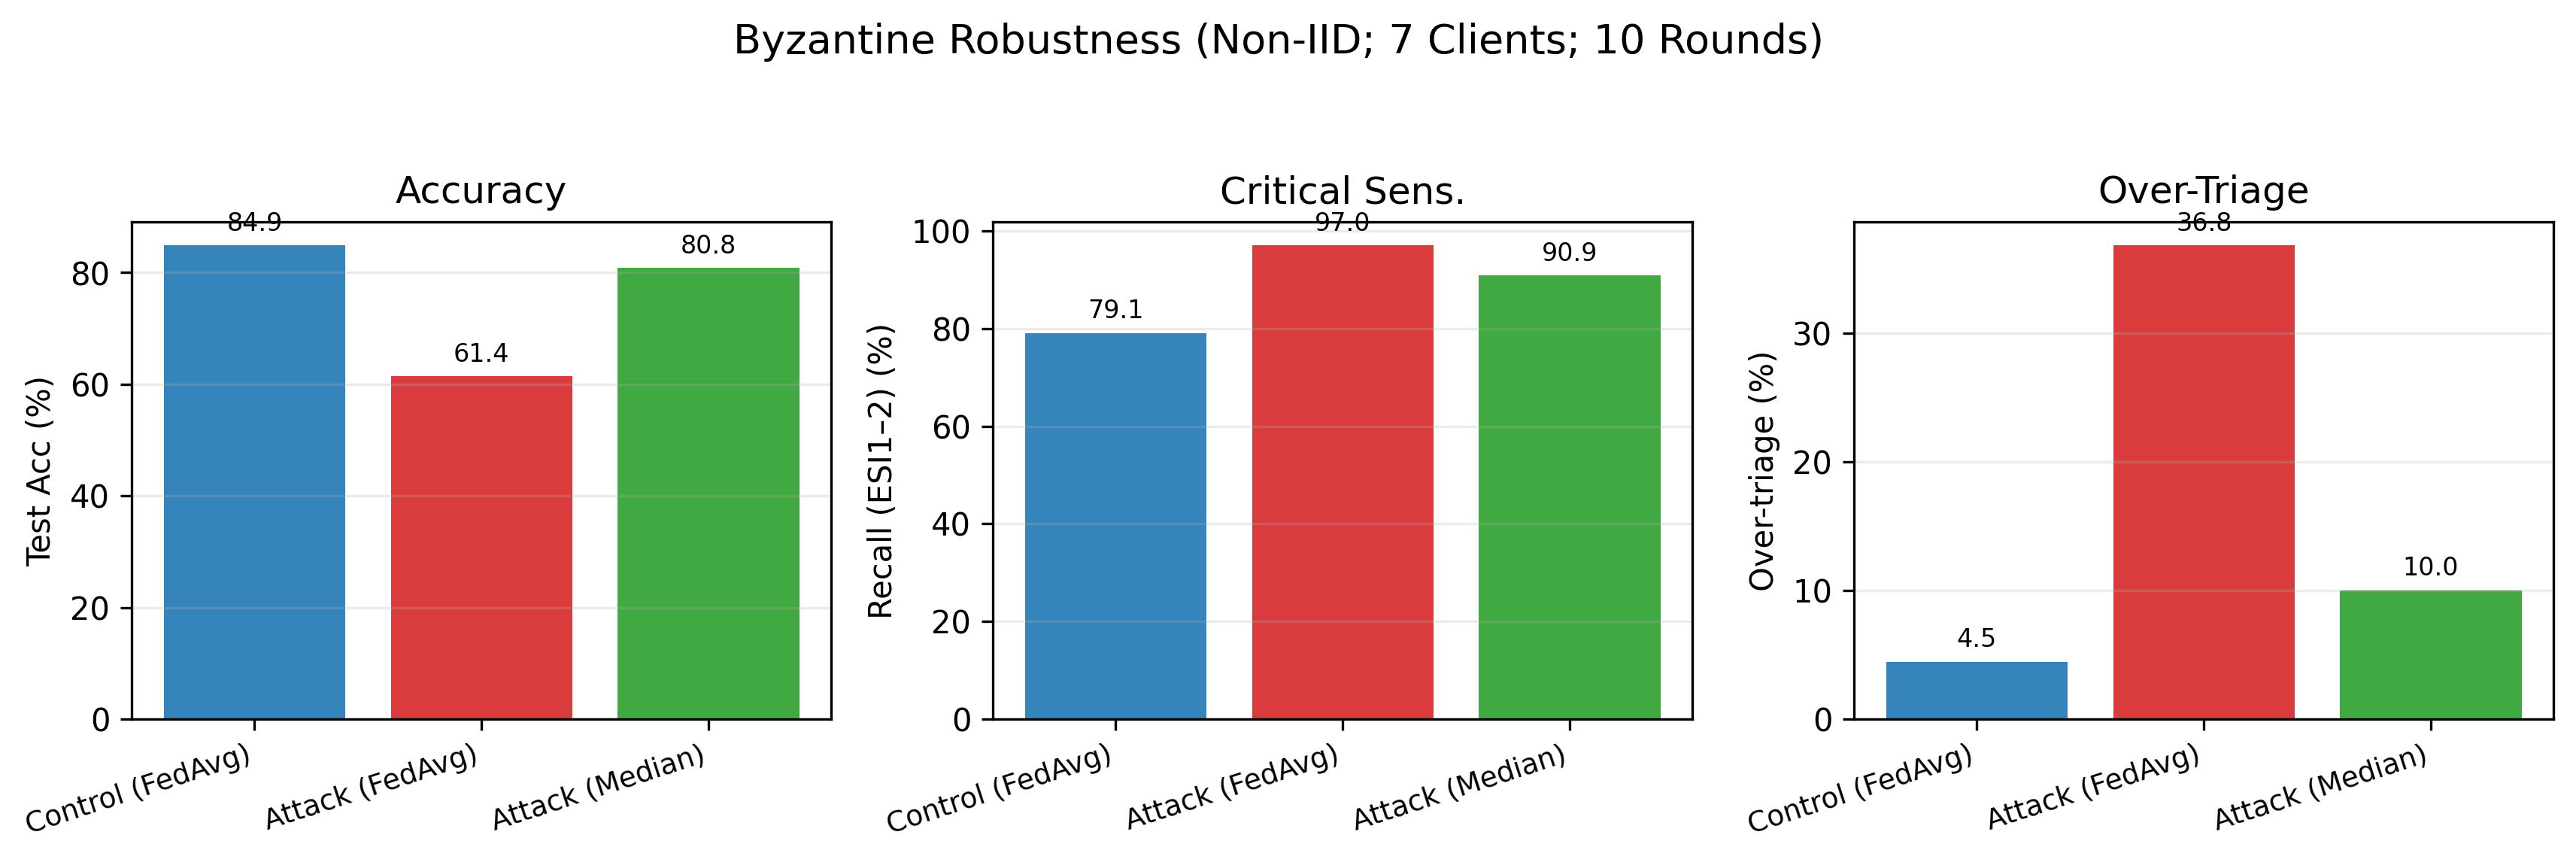
\includegraphics[width=0.9\textwidth]{figures/byzantine_robustness.png}
\caption{Byzantine robustness evaluation (non-IID; 7 clients; 10 rounds). Under a poisoning attack, FedAvg exhibits a large accuracy drop and severe over-triage, while median aggregation recovers utility and reduces attack-induced over-triage.}
\label{fig:byzantine}
\end{figure}

\subsection{Calibration Quality and Reliability}

Figures~\ref{fig:acc-f1-rounds} and \ref{fig:reliability} report validation utility (accuracy and macro-F1) and calibration metrics (ECE and NLL) across rounds for cross-silo FL (by-site, non-DP). The red-focus model attains higher validation utility and improved calibration by the final round (ECE 0.040 vs.\ 0.086 for the flat baseline), indicating that safety-focused modeling can improve both utility and reliability in this setting.

To summarize test-time reliability, Table~\ref{tab:reliability-metrics} reports NLL, ECE, and Brier score on the held-out test set across the core systems. The red-focus FL model improves calibration relative to flat FL (NLL 0.361 vs.\ 0.442; ECE 0.036 vs.\ 0.086), while DP-SGD degrades reliability (NLL 0.521; ECE 0.102) despite high overall accuracy, consistent with the extreme-class failure in ESI-1.

\begin{table}[H]
\centering
\caption{Test-set reliability metrics (lower is better). ECE uses 10 bins.}
\label{tab:reliability-metrics}
\small
\begin{tabular}{lccc}
\toprule
System & NLL & ECE & Brier \\
\midrule
HistGB (centralized) & 0.242 & 0.004 & 0.027 \\
Centralized NN (non-DP) & 0.326 & 0.041 & 0.035 \\
FL Flat (non-DP; 3 sites, 20 rounds) & 0.442 & 0.086 & 0.047 \\
FL Red-Focus (non-DP; 3 sites, 20 rounds) & 0.361 & 0.036 & 0.039 \\
DP-SGD (3 sites, 5 rounds; $\sigma=1.0$; Adam) & 0.521 & 0.102 & 0.050 \\
\bottomrule
\end{tabular}
\end{table}

\begin{figure}[H]
\centering
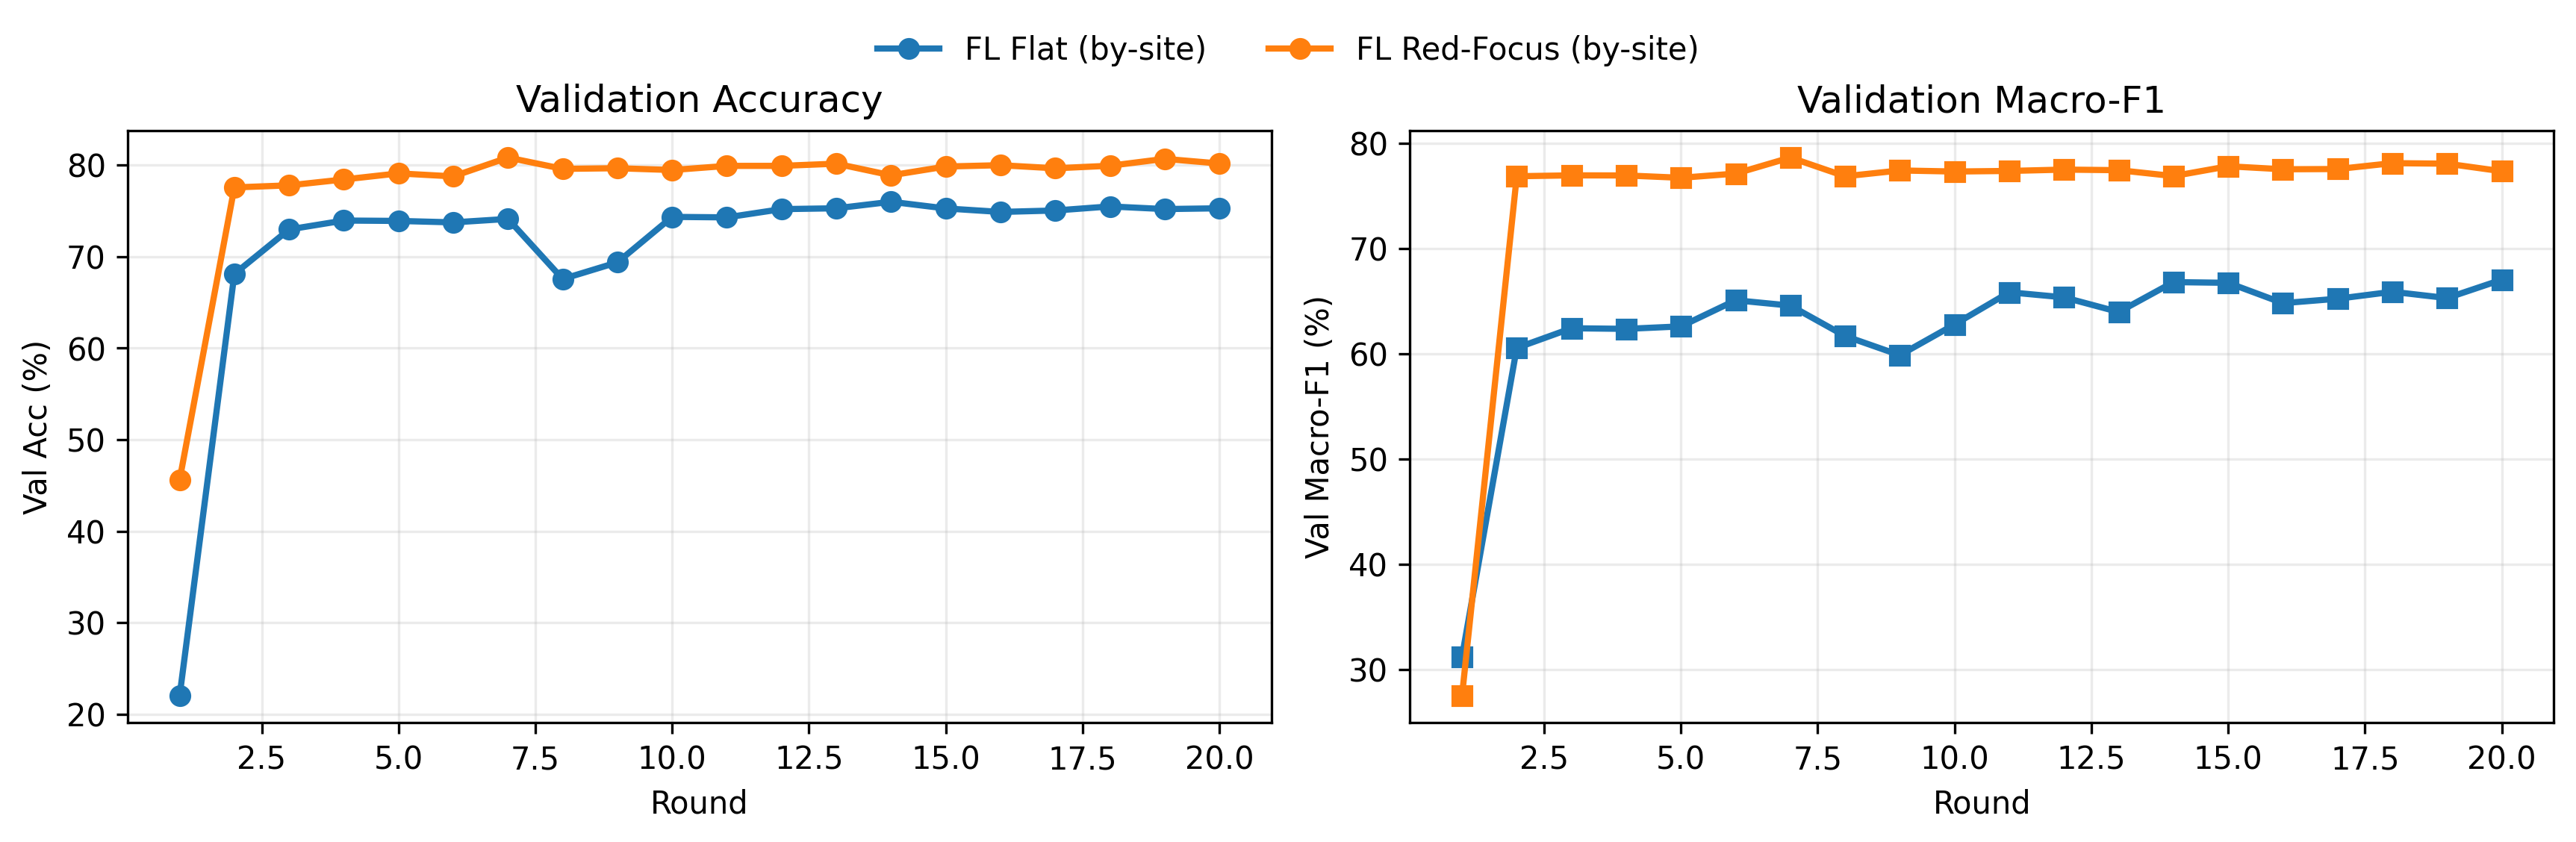
\includegraphics[width=0.8\textwidth]{figures/fl_advanced_acc_f1_vs_rounds.png}
\caption{Validation accuracy and macro-F1 across rounds for cross-silo FL (by-site, non-DP), comparing the flat FedAvg baseline to the red-focus hierarchical model.}
\label{fig:acc-f1-rounds}
\end{figure}

\begin{figure}[H]
\centering
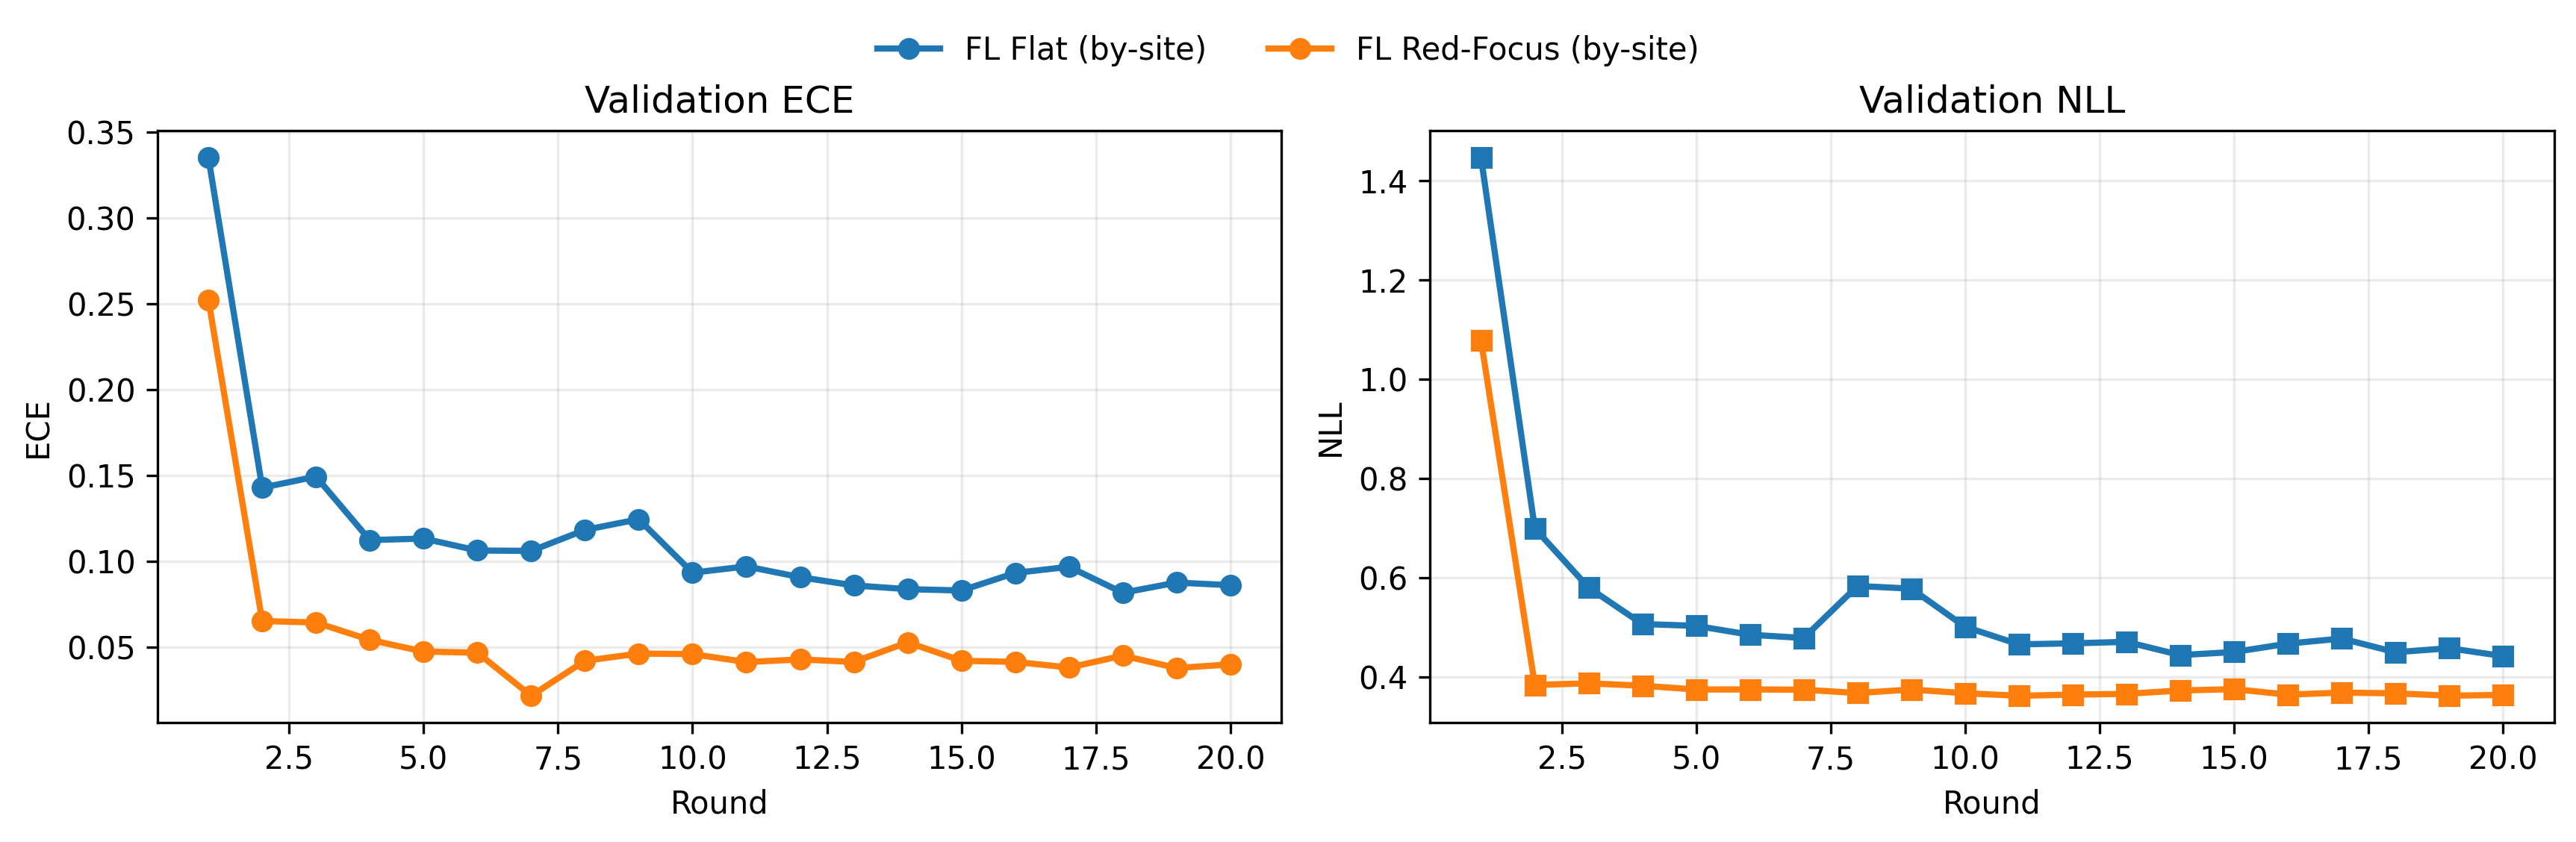
\includegraphics[width=0.8\textwidth]{figures/fl_advanced_ece_nll_vs_rounds.png}
\caption{Validation calibration metrics (ECE and NLL) across rounds for cross-silo FL (by-site, non-DP).}
\label{fig:reliability}
\end{figure}

Well-calibrated probabilities are essential for clinical decision-making. A predicted probability of 80\% for ESI-2 should correspond to an actual frequency of approximately 80\% in the validation data. This enables clinicians to trust the model's confidence scores and set evidence-based thresholds.

\subsection{Fairness and Interpretability}

Our codebase reports subgroup metrics by age group and gender (accuracy, weighted F1, and predicted critical-rate diagnostics) and supports optional SHAP analysis for global feature attributions. Across systems, we observe substantial differences in \emph{predicted} critical rates across age groups, which likely reflects both real case-mix differences and model behavior; we therefore treat these subgroup outputs as descriptive deployment diagnostics rather than a normative fairness guarantee. A more complete fairness assessment for triage should emphasize clinically meaningful notions such as equal opportunity for the critical band (ESI-2/ESI-1) and should be evaluated prospectively across institutions. We leave a comprehensive interpretability and fairness analysis of the best-performing non-DP systems as future work.

\subsection{Communication Efficiency}

Each client communicates roughly one model upload and download per round. In our cross-silo FL experiments (3 sites/clients), the total communication per round is approximately 1.63--1.68~MB (about 0.54--0.56~MB per client per round, uplink+downlink), reflecting the 0.27--0.28~MB model footprint. In the 7-client robustness experiments, total communication is approximately 3.80--3.92~MB per round under the same accounting model. This low bandwidth requirement supports deployment in resource-constrained edge environments.

\begin{figure}[H]
\centering
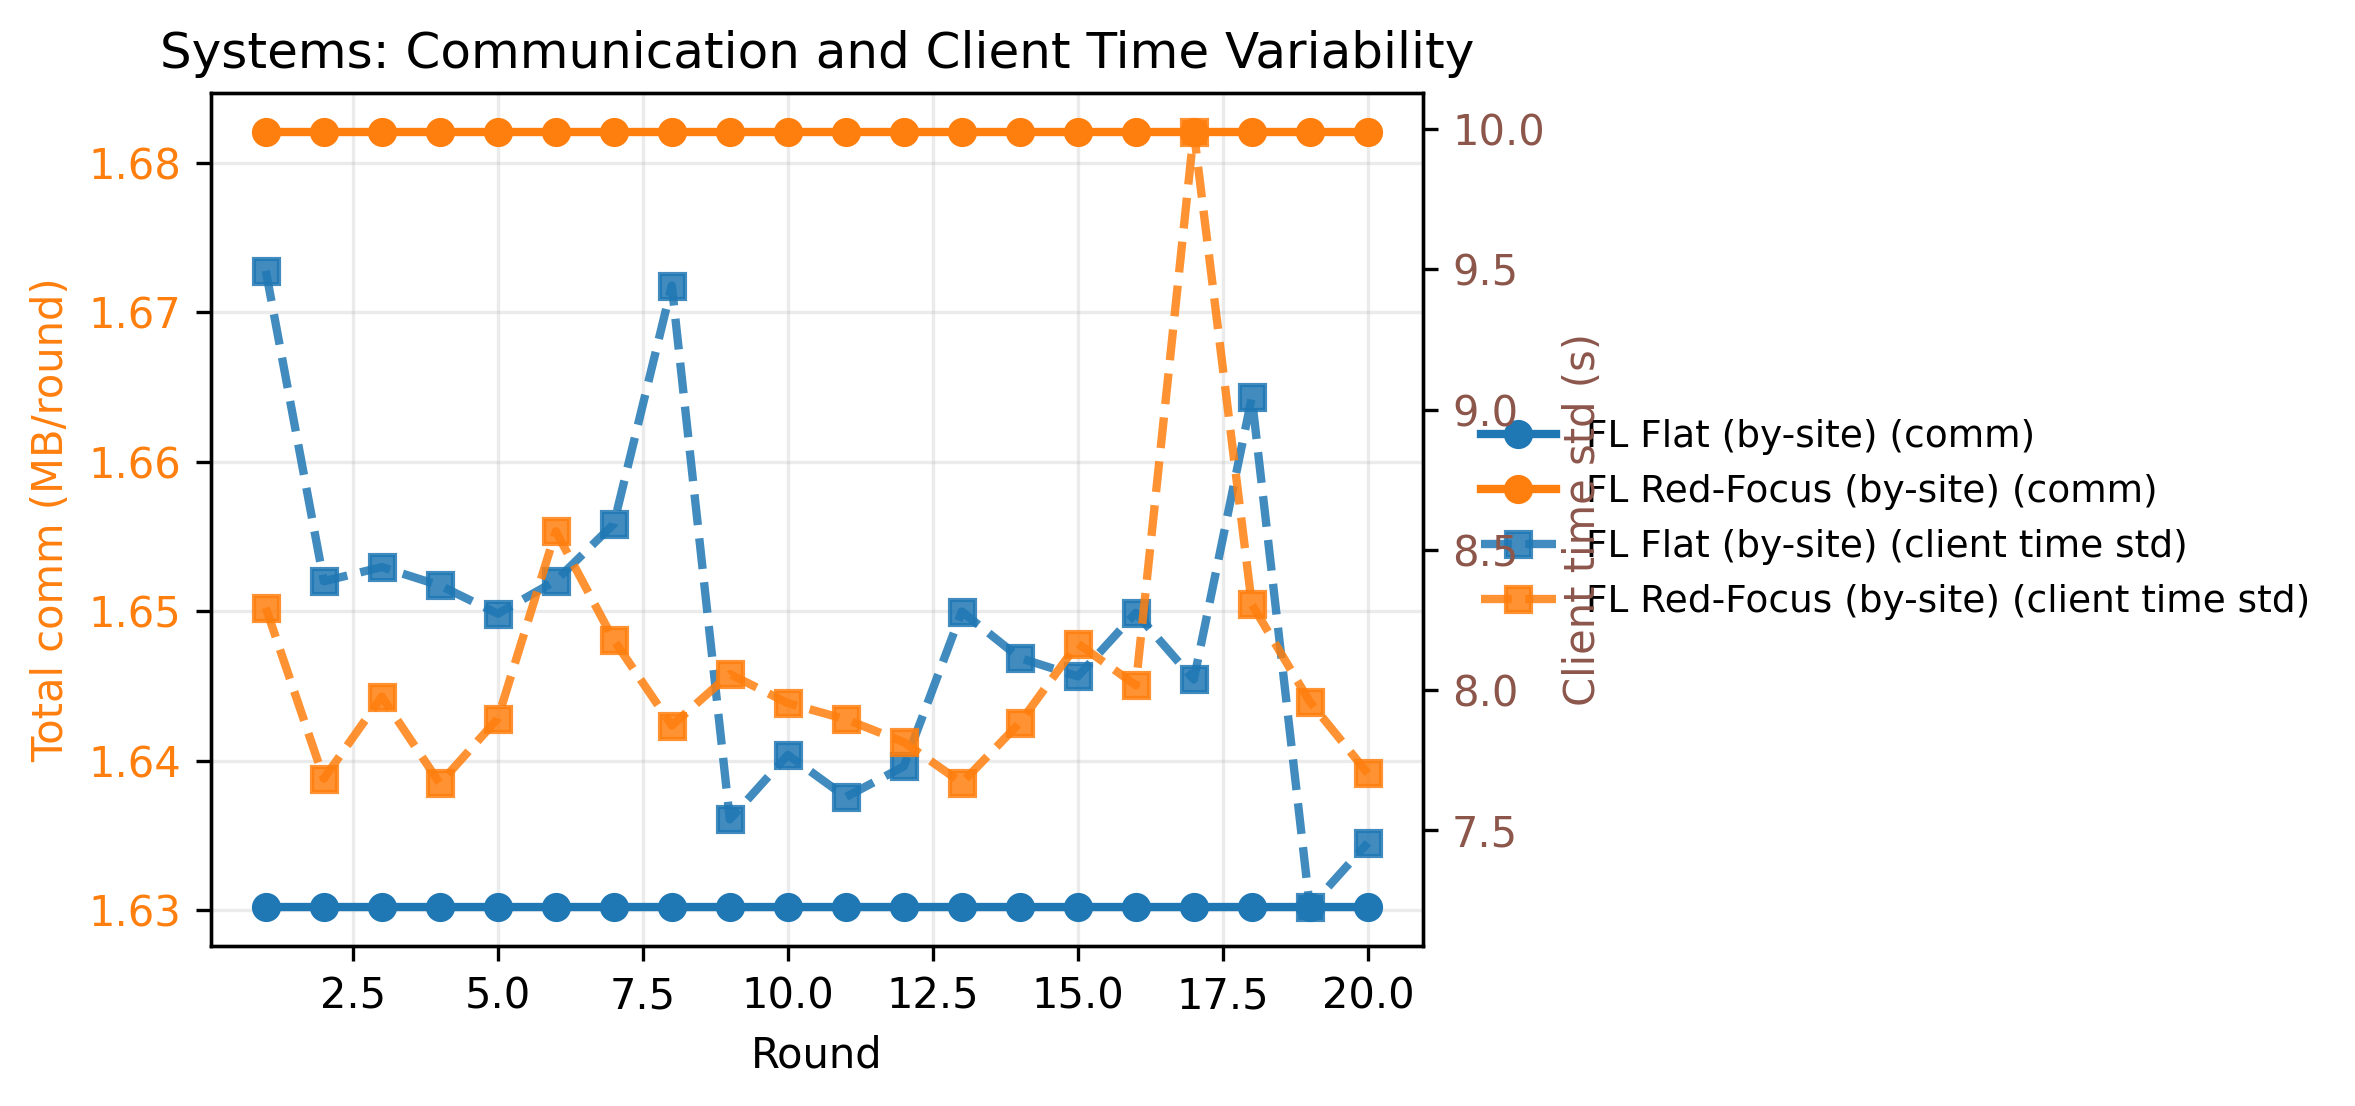
\includegraphics[width=0.8\textwidth]{figures/fl_advanced_systems_vs_rounds.png}
\caption{Systems metrics across rounds for cross-silo FL (by-site, non-DP). Communication is reported as MB per round (total bytes exchanged across all clients, uplink+downlink; 1~MB = $10^6$ bytes). Under our accounting model, communication is constant across rounds because the model size is constant; client-time standard deviation varies across rounds due to heterogeneous local training times.}
\label{fig:systems}
\end{figure}

%%%%%%%%%%%%%%%%%%%%%%%%%%%%%%%%%%%%%%%%%%
\section{Discussion}\label{sec:discussion}

\subsection{Security and Privacy Implications}

Federated learning reduces direct data exposure by keeping patient records on-site, but it is not inherently private \cite{zhu2019deep,shokri2017}. In our pipeline, privacy and integrity are addressed through optional client-side DP-SGD \cite{dwork2006,abadi2016deep,yousefpour2021opacus}, robust aggregation options \cite{yin2018byzantine}, and standard secure transport (TLS). DP-SGD provides formal privacy guarantees, but our DP ablation demonstrates that achieving strong privacy can substantially degrade extreme-class performance in multi-class triage (ESI-1 recall 0.0). Robust aggregators (median/trimmed-mean) are implemented to mitigate outliers, and we empirically validate median aggregation under simulated Byzantine clients. Secure aggregation can be integrated to reduce server visibility into individual updates \cite{bonawitz2017}; however, secure aggregation is not enabled in our current experiments.

Despite these measures, some challenges remain. Our approach assumes an honest-but-curious server, which follows the protocol but may be curious. Fully malicious servers would require cryptographic secure aggregation or trusted execution environments. Additionally, while our robust aggregation provides basic defense, sophisticated adversaries with multiple compromised clients could potentially evade statistical filters. Future work will need to evaluate defenses against state-of-the-art poisoning attacks. Even with DP, there is a risk of privacy leakage through auxiliary information, such as public demographic data, which could enable inference attacks. Therefore, privacy-utility trade-offs must be carefully tuned for each deployment context. In the future, we plan to implement full secure aggregation to eliminate the reliance on the honest-but-curious assumption and to evaluate robustness against targeted poisoning attacks using techniques from recent adversarial federated learning research.

\subsection{Federated Learning Challenges and Solutions}

Data heterogeneity is a significant challenge in federated learning, as non-IID data distributions across clients can degrade performance \cite{hsu2019measuring}. Hospitals naturally have different patient populations, case mixes, and data collection practices. Our hierarchical critical-first (hierarchical) model partially mitigates this issue through specialized heads that adapt to local critical-band distributions. Future work will explore per-client personalization, such as FedPer \cite{arivazhagan2019}, and heterogeneous optimization methods such as FedProx \cite{li2020fedprox}, as well as meta-learning and adaptive aggregation weights.

Communication efficiency is another important consideration. Our small model size (0.27--0.28~MB) minimizes communication overhead. For larger models, techniques such as gradient compression, sparsification, or federated distillation could further reduce bandwidth requirements.

Finally, convergence in federated training typically requires more rounds than in centralized training. Our cross-silo non-DP experiments use 20 rounds, while the DP ablation uses 5 rounds; production systems may require substantially more communication rounds. Adaptive learning rates and momentum-based aggregation, such as FedAvgM, can help accelerate convergence.

\subsection{Clinical Deployment Considerations}

For real-world deployment, the model must be seamlessly integrated into ED triage workflows. This requires several considerations. First, our lightweight architecture supports real-time inference with a latency of less than 100ms on standard hospital servers. Second, SHAP explanations provide feature-level insights that clinicians can validate against their domain knowledge, enhancing explainability. Third, the model's predictions should augment, not replace, clinical judgment, with clinicians retaining final decision-making authority in a human-in-the-loop system. Finally, continuous performance monitoring, drift detection, and audit logs are necessary to ensure the model's reliability over time. A comprehensive model card, detailing the intended use, limitations, and performance characteristics, will accompany the open-source release to promote transparency.

Federated learning with differential privacy aligns well with the requirements of HIPAA and GDPR by minimizing data movement and providing formal privacy guarantees. However, regulatory approval, such as FDA clearance, will require extensive validation, prospective clinical trials, and thorough documentation of safety and efficacy.

Fairness and safety must be monitored continuously, especially on rare subgroups and rare acuity levels. While federated learning can broaden population coverage by incorporating multiple institutions, specialized validation remains essential before deployment.

\subsection{Comparison to Centralized Training}

The strongest centralized baseline (HistGB, 89.5\% accuracy) outperforms our federated red-focus model (80.5\% accuracy) in overall accuracy. Centralized training, however, requires pooling patient data, which may violate privacy regulations in many jurisdictions, creates security risks from centralized data breaches, and limits participation from institutions that are unwilling to share their data.

Our federated approach offers significant privacy advantages that, in our view, can outweigh moderate differences in accuracy. The performance gap can be further narrowed by increasing the number of communication rounds, implementing personalization with client-specific final layers adapted to local distributions, using advanced aggregation techniques such as weighted averaging based on client data quality or confidence, or employing hybrid approaches that combine federated pre-training with local fine-tuning.

\subsection{Limitations}

Our evaluation is based on a single public dataset. Real-world federated deployments will involve multiple institutions with distinct electronic health record systems, coding practices, and patient populations, so multi-site prospective validation is needed. Additionally, our model uses tabular features, including vitals, labs, and demographics. Incorporating chief-complaint text, clinical notes, or time-series physiological signals could improve performance, especially in ambiguous cases.

While we implement robust aggregation and evaluate a basic poisoning scenario, we do not evaluate the system against targeted backdoor attacks or adaptive adversaries. A comprehensive adversarial evaluation is an important area for future work. In addition, while we implement composed R\'enyi DP accounting across rounds for our DP-SGD runs, the DP model still fails on the rarest acuity class (ESI-1), so improving DP extreme-class utility remains an open challenge. Finally, we simulate federated learning in a controlled environment. A production deployment would require secure communication infrastructure, identity management, access control, and compliance with institutional IT policies.

%%%%%%%%%%%%%%%%%%%%%%%%%%%%%%%%%%%%%%%%%%
\section{Conclusions}\label{sec:conclusion}

We presented a federated learning framework for emergency department triage that demonstrates how Edge AI techniques can enable collaborative model development while reducing direct data sharing. On ESI-5, our centralized neural model achieves 85.4\% test accuracy with 95.3\% critical-band sensitivity, while a strong tabular baseline (HistGB) reaches 89.5\% accuracy. In cross-silo FL using three real sites, a red-focus hierarchical model reaches 80.5\% accuracy and 90.8\% critical sensitivity, improving safety metrics relative to a flat FedAvg baseline. We also empirically validate robust aggregation: under a poisoning attack, FedAvg suffers a large accuracy drop and severe over-triage, while median aggregation recovers much of the utility and reduces over-triage. In contrast, our DP-SGD ablation (3 sites, 5 rounds; $\varepsilon\approx1.15$, $\delta=10^{-5}$) maintains high overall accuracy but fails on ESI-1 (0.0 recall), reducing macro-F1 and critical sensitivity.

These findings highlight that (i) safety-focused objectives can partially close the performance gap under federation, but (ii) strong formal differential privacy and robust deployment under adaptive adversaries remain open challenges. Future work will explore stronger personalization, longer training horizons, secure aggregation, and improved privacy-aware optimization to move toward clinically reliable, privacy-preserving federated triage.

Future work will explore several directions. First, we plan to integrate full cryptographic secure aggregation protocols to eliminate the honest-but-curious server assumption. Second, we will evaluate robustness against targeted poisoning and backdoor attacks. Third, we will pursue multi-site prospective validation with real hospital deployments. Fourth, we will incorporate clinical text and time-series data for richer representations. Fifth, we will investigate personalization techniques, such as FedPer and meta-learning, to better handle non-IID data. Finally, we will work on privacy-utility optimization through advanced DP mechanisms, such as adaptive clipping and privacy amplification.

Our open-source release provides a complete toolkit for privacy-preserving federated triage, enabling the research community to build on this foundation and advance secure Edge AI for healthcare.

%%%%%%%%%%%%%%%%%%%%%%%%%%%%%%%%%%%%%%%%%%
\vspace{6pt}

%%%%%%%%%%%%%%%%%%%%%%%%%%%%%%%%%%%%%%%%%%
\authorcontributions{Conceptualization, C.B.B.; methodology, C.B.B.; software, C.B.B.; validation, C.B.B.; formal analysis, C.B.B.; investigation, C.B.B.; resources, C.B.B.; data curation, C.B.B.; writing---original draft preparation, C.B.B.; writing---review and editing, C.B.B.; visualization, C.B.B.; project administration, C.B.B. The author has read and agreed to the published version of the manuscript.}

\funding{This research received no external funding.}

\institutionalreview{Not applicable. This study uses publicly available de-identified data.}

\informedconsent{Not applicable. This study uses publicly available de-identified data.}

\dataavailability{The public triage dataset used in this study is available on Kaggle (\url{https://www.kaggle.com/datasets/maalona/hospital-triage-and-patient-history-data}). Results are reported on this public dataset, and our code is released under a permissive license (MIT), but no redistribution of the dataset is included. Code is available at: \url{https://github.com/cenab/triaj-research}.}

\acknowledgments{The author thanks the open-source community for tools including PyTorch, Opacus, scikit-learn, and the federated learning research community for foundational work that enabled this study.}

\conflictsofinterest{The author declares no conflicts of interest.}

%%%%%%%%%%%%%%%%%%%%%%%%%%%%%%%%%%%%%%%%%%
\abbreviations{Abbreviations}{
The following abbreviations are used in this manuscript: AI (Artificial Intelligence), DCA (Decision Curve Analysis), DP (Differential Privacy), DP-SGD (Differentially Private Stochastic Gradient Descent), ECE (Expected Calibration Error), ED (Emergency Department), ESI (Emergency Severity Index), FL (Federated Learning), GDPR (General Data Protection Regulation), HIPAA (Health Insurance Portability and Accountability Act), MLP (Multi-Layer Perceptron), NLL (Negative Log-Likelihood), NP (Neyman-Pearson), PHI (Protected Health Information), SHAP (SHapley Additive exPlanations), and TLS (Transport Layer Security).
}

%%%%%%%%%%%%%%%%%%%%%%%%%%%%%%%%%%%%%%%%%%
\begin{adjustwidth}{-\extralength}{0cm}

\reftitle{References}

% ACS format references
\begin{thebibliography}{999}

\bibitem{cdc2022}
Centers for Disease Control and Prevention. National Hospital Ambulatory Medical Care Survey: 2022 National Summary Tables. Available online: \url{https://www.cdc.gov/nchs/data/nhamcs/web_tables/2022-nhamcs-ed-web-tables.pdf} (accessed on 11 November 2025).

\bibitem{voigt2017}
Voigt, P.; von dem Bussche, A. \textit{The EU General Data Protection Regulation (GDPR): A Practical Guide}; Springer: Cham, Switzerland, 2017.

\bibitem{mcmahan2017}
McMahan, H.B.; Moore, E.; Ramage, D.; Hampson, S.; Arcas, B.A. Communication-efficient learning of deep networks from decentralized data. In \textit{Proc. AISTATS}, PMLR, 2017; pp. 1273--1282.

\bibitem{kairouz2021}
Kairouz, P.; McMahan, H.B.; et al. Advances and open problems in federated learning. \textit{Found. Trends Mach. Learn.} \textbf{2021}, \textit{14}, 1--210.

\bibitem{zhu2019deep}
Zhu, L.; Liu, Z.; Han, S. Deep leakage from gradients. In \textit{Proc. NeurIPS}, 2019; pp. 14747--14756.

\bibitem{shokri2017}
Shokri, R.; Stronati, M.; Song, C.; Shmatikov, V. Membership inference attacks against machine learning models. In \textit{Proc. IEEE S\&P}, 2017; pp. 3--18.

\bibitem{blanchard2017}
Blanchard, P.; El Mhamdi, E.M.; Guerraoui, R.; Stainer, J. Machine learning with adversaries: Byzantine tolerant gradient descent. In \textit{Proc. NeurIPS}, 2017; pp. 119--129.

\bibitem{yin2018byzantine}
Yin, D.; Chen, Y.; Kannan, R.; Bartlett, P. Byzantine-robust distributed learning: Towards optimal statistical rates. In \textit{Proc. ICML}, PMLR, 2018; pp. 5650--5659.

\bibitem{raita2019}
Raita, Y.; Goto, T.; Faridi, M.K.; Brown, D.F.M.; Camargo Jr., C.A.; Hasegawa, K. Emergency department triage prediction of clinical outcomes using machine learning models. \textit{Crit. Care} \textbf{2019}, \textit{23}, 64.

\bibitem{levin2018}
Levin, S.; Toerper, M.; Hamrock, E.; et al. Machine-learning-based electronic triage more accurately differentiates patients with respect to clinical outcomes compared with the emergency severity index. \textit{Ann. Emerg. Med.} \textbf{2018}, \textit{71}, 565--574.

\bibitem{liu2021_sci_rep}
Liu, Y.; Gao, J.; Liu, J.; et al. Development and validation of a practical machine-learning triage algorithm for the detection of patients in need of critical care in the emergency department. \textit{Sci. Rep.} \textbf{2021}, \textit{11}, 24044.

\bibitem{chang2024_bmc}
Chang, Y.-H.; Lin, Y.-C.; Huang, F.-W.; et al. Using machine learning and natural language processing in triage for prediction of clinical disposition in the emergency department. \textit{BMC Emerg. Med.} \textbf{2024}, \textit{24}, 237.

\bibitem{gligorijevic2018}
Gligorijevic, D.; Stojanovic, J.; Satz, W.; et al. Deep Attention Model for Triage of Emergency Department Patients. \textit{arXiv} \textbf{2018}, arXiv:1804.03240.

\bibitem{vickers2006}
Vickers, A.J.; Elkin, E.B. Decision curve analysis: A novel method for evaluating prediction models. \textit{Med. Decis. Making} \textbf{2006}, \textit{26}, 565--574.

\bibitem{araf2024_csl_review}
Araf, I.; Ayon, S.I.; Rahman, A. Cost-sensitive learning for imbalanced medical data: A review. \textit{Artif. Intell. Rev.} \textbf{2024}, \textit{57}, 1--42.

\bibitem{pes2021_cost_sens_med}
Pes, B.; Ruiu, A.P.; Cossu, G.; Angioni, G. Cost-sensitive learning strategies for high-dimensional and imbalanced medical data. \textit{BMC Med. Inform. Decis. Mak.} \textbf{2021}, \textit{21}, 1--19.

\bibitem{tong2013_np}
Tong, X. A Plug-in Approach to Neyman-Pearson Classification. \textit{J. Mach. Learn. Res.} \textbf{2013}, \textit{14}, 3011--3040.

\bibitem{guo2017}
Guo, C.; Pleiss, G.; Sun, Y.; Weinberger, K.Q. On calibration of modern neural networks. In \textit{Proc. ICML}, PMLR, 2017; pp. 1321--1330.

\bibitem{ovadia2019}
Ovadia, Y.; Fertig, E.; Ren, J.; et al. Can you trust your model's uncertainty? Evaluating predictive uncertainty under dataset shift. In \textit{Proc. NeurIPS}, 2019; pp. 13991--14002.

\bibitem{yu2022_mdt}
Yu, Y.; Ma, J.; Zhao, H.; Vasconcelos, N. Robust Calibration with Multi-domain Temperature Scaling. In \textit{Proc. NeurIPS}, 2022; Vol. 35, pp. 10526--10539.

\bibitem{rieke2020}
Rieke, N.; et al. The future of digital health with federated learning. \textit{NPJ Digit. Med.} \textbf{2020}, \textit{3}, 119.

\bibitem{sheller2020}
Sheller, M.J.; et al. Federated learning in medicine: Facilitating multi-institutional collaborations without sharing patient data. \textit{Sci. Rep.} \textbf{2020}, \textit{10}, 12598.

\bibitem{dayan2021}
Dayan, I.; Roth, H.; Zhong, A.; et al. Federated learning for predicting clinical outcomes in patients with COVID-19. \textit{Nat. Med.} \textbf{2021}, \textit{27}, 1735--1743.

\bibitem{teo2024_fl_survey}
Teo, Z.L.; Jin, L.; Li, S.; Miao, D.; Ting, D.S.W. Federated machine learning in healthcare: A systematic review on clinical applications and technical architecture. \textit{Cell Rep. Med.} \textbf{2024}, \textit{5}, 101419.

\bibitem{peng2024_fedcal}
Peng, H.; Wang, W.; Chen, F.; et al. FedCal: Achieving Local and Global Calibration in Federated Learning via Aggregated Parameterized Scaler. In \textit{Proc. ICML}, PMLR, 2024; Vol. 235, pp. 39856--39880.

\bibitem{dwork2006}
Dwork, C. Differential Privacy. In \textit{Proc. ICALP}, Springer: Berlin/Heidelberg, Germany, 2006; pp. 1--12.

\bibitem{abadi2016deep}
Abadi, M.; Chu, A.; Goodfellow, I.; McMahan, H.B.; Mironov, I.; Talwar, K.; Zhang, L. Deep learning with differential privacy. In \textit{Proc. ACM CCS}, 2016; pp. 308--318.

\bibitem{mironov2017}
Mironov, I. R\'enyi differential privacy. In \textit{Proc. IEEE CSF}, 2017; pp. 263--275.

\bibitem{yousefpour2021opacus}
Yousefpour, A.; Shilov, I.; Sablayrolles, A.; Testuggine, D.; Prasad, K.; Malek, M.; Nguyen, J.; Ghosh, S.; Bharadwaj, A.; Zhao, J.; et al. Opacus: User-Friendly Differential Privacy Library in PyTorch. \textit{arXiv} \textbf{2021}, arXiv:2109.12298.

\bibitem{bu2020}
Bu, Z.; Dong, J.; Long, Q.; Su, W.J. Deep learning with Gaussian differential privacy. \textit{Harv. Data Sci. Rev.} \textbf{2020}, \textit{2}, DOI:10.1162/99608f92.cfc5dd25.

\bibitem{bonawitz2017}
Bonawitz, K.; Ivanov, V.; Kreuter, B.; Marcedone, A.; McMahan, H.B.; Patel, S.; Ramage, D.; Segal, A.; Seth, K. Practical Secure Aggregation for Privacy-Preserving Machine Learning. In \textit{Proc. ACM CCS}, 2017; pp. 1175--1191.

\bibitem{zhang2020}
Zhang, C.; Li, S.; Xia, J.; Wang, W.; Yan, F.; Liu, Y. BatchCrypt: Efficient Homomorphic Encryption for Cross-Silo Federated Learning. In \textit{Proc. USENIX ATC}, 2020; pp. 493--506.

\bibitem{lundberg2017}
Lundberg, S.M.; Lee, S.-I. A unified approach to interpreting model predictions. In \textit{Proc. NeurIPS}, 2017; pp. 4765--4774.

\bibitem{ribeiro2016}
Ribeiro, M.T.; Singh, S.; Guestrin, C. ``Why should I trust you?'' Explaining the predictions of any classifier. In \textit{Proc. ACM KDD}, 2016; pp. 1135--1144.

\bibitem{hardt2016}
Hardt, M.; Price, E.; Srebro, N. Equality of opportunity in supervised learning. In \textit{Proc. NeurIPS}, 2016; pp. 3315--3323.

\bibitem{mohri2019agnostic}
Mohri, M.; Sivek, G.; Suresh, A.T. Agnostic Federated Learning. In \textit{Proc. ICML}, PMLR, 2019; pp. 4615--4625.

\bibitem{lin2017}
Lin, T.-Y.; Goyal, P.; Girshick, R.; He, K.; Doll\'ar, P. Focal loss for dense object detection. In \textit{Proc. ICCV}, 2017; pp. 2980--2988.

\bibitem{hsu2019measuring}
Hsu, T.M.H.; Qi, H.; Brown, M. Measuring the effects of non-identical data distribution for federated visual classification. \textit{arXiv} \textbf{2019}, arXiv:1909.06335.

\bibitem{arivazhagan2019}
Arivazhagan, M.G.; Aggarwal, V.; Singh, A.K.; Choudhary, S. Federated Learning with Personalization Layers. \textit{arXiv} \textbf{2019}, arXiv:1912.00818.

\bibitem{li2020fedprox}
Li, T.; Sahu, A.K.; Zaheer, M.; Sanjabi, M.; Talwalkar, A.; Smith, V. Federated Optimization in Heterogeneous Networks. In \textit{Proc. MLSys}, 2020; Vol. 2, pp. 429--450.

\end{thebibliography}

\end{adjustwidth}

\PublishersNote{}
\end{document}
